\documentclass[11pt]{article}
\usepackage[a4paper,margin=1in]{geometry}
\usepackage[T1]{fontenc}
\usepackage[utf8]{inputenc}
\usepackage{lmodern}
\usepackage{microtype}
\usepackage{amsmath,amssymb}
\usepackage{graphicx}
\usepackage{booktabs}
\usepackage{multirow}
\usepackage{xcolor}
\usepackage{hyperref}
\usepackage[numbers,sort&compress]{natbib}
\usepackage{caption}
\usepackage{subcaption}
\usepackage{enumitem}
\usepackage{float}
\usepackage{adjustbox}
\usepackage{longtable}
\usepackage{textcomp}
\hypersetup{colorlinks=true,linkcolor=blue!50!black,citecolor=blue!50!black,urlcolor=blue!50!black}
\captionsetup{font=small,labelfont=bf}
\graphicspath{{figures/}}
\setlength{\parskip}{0.25em}
\newcommand{\dsurp}{surprise}
\newcommand{\dconn}{connection}
\newcommand{\dcoh}{coherence}
\newcommand{\ci}[2]{[#1,\,#2]}
\newcommand{\todo}[1]{\textcolor{red}{[#1]}}

\title{Where Creativity Lives in a Language Model:\\
Not the Sampler, Not the Prompt, but Interrupting the Loop}
\author{Roberto Isamu Ono Filho\\
Independent researcher\\
\texttt{ono.roberto@gmail.com}}
\date{Preprint, \today}

\begin{document}
\maketitle

\begin{abstract}
Where does the novelty a language model can produce with no task come from?
We test the three places usually credited, the sampler, the prompt and the
loop, on base models, with an LLM judge that is itself measured. An
entropy-banded anti-probable decoder roughly doubles $n$-gram novelty against
the training corpus but shows no detectable effect on judged surprise or
connection; input improbability shows no benefit under the
operationalizations we tested. The loop is different. Forced to continue a
premise with the end-of-text token masked, a base model degenerates into
repetitive modes; a closed loop built on the architecture of spontaneous
cognition revives it, and taking that loop apart over 23 conditions locates
most of the effect in two simple operations: a windowed repetition penalty
(habituation) and a periodic \emph{interruption}, one neutral sentence
injected every few hundred tokens. On windows of generated text only, judged
by Claude Opus~5 ($k=5$) with the premise as the unit ($n=10$), the
interruption raises surprise from 1.6 to 3.0 and connection from 1.3 to 3.7
over habituation alone (paired permutation $p=0.002$) and matches the full
scaffold. Part of that is self-copy: given the same four sentences in
rotation, the model replays its own earlier segments, out of the judge's
view; on fresh windows the interruption adds +1.2 to +1.4 surprise and
+0.8 connection, and a reset context, which cannot replay, adds +1.9 and
+2.0. Controls show what carries the effect: a bare paragraph break does
nothing and a continuity connective hurts; the new subject carries most of
it; injecting the premise or the stream's own past is as bad as not
interrupting; salience timing is no better than a clock. The gains are local:
judged as whole documents, no arm builds an integrated text. A pre-registered replication on ten new premises confirms
the primary contrast ($p=0.003$) and refutes the expectation that the kept
context carries connection. The ordering replicates
on three base models from two families, under a second judge family and in
the rankings of independent human readers. These results characterize a
simple, controllable intervention for forced open-ended generation; they do
not establish a general mechanism of creativity.

\end{abstract}

\section{Introduction}

Ask a language model for something new and you will usually get something
fluent, plausible and familiar. Three places are commonly blamed, and three
places are commonly optimized. The first is the \emph{sampler}: the tail of
the next-token distribution, tamed by nucleus, typical or min-$p$ truncation,
or courted by higher temperature. The second is the \emph{prompt}: the
input, engineered to steer the model somewhere it would not go on its own.
The third, less often, is the \emph{loop}: what happens when a model's output
becomes its own next input and nobody asks anything.

The loop is where human novelty is usually placed. Insight rarely arrives as
the answer to a strange question. It arises inside a closed circuit of
thought feeding on its own output, during incubation, mind-wandering and
sleep, when a spontaneously generated deviation survives critical review and
is linked back to what came before. The neuroscience of creative cognition
describes three coupled systems: a default-mode network that generates, an
executive network that evaluates, and a salience network that decides what
deserves attention. More creative people show more coupling between the
first two, with salience regions coupling first
\citep{beaty2016dynamics,beaty2018robust}. Creativity itself is often
characterized as connecting semantically distant concepts
\citep{kenett2018semantic}, and incubation, leaving a problem and coming back
to it, has a measured effect on solving it \citep{sio2009incubation}.

This paper asks, with controls, where the novelty a base language model
produces with no task comes from, and which of the operations usually
credited for it survive measurement. The outcome we measure is narrow and we
name it as such: \emph{judged narrative surprise, connection and coherence}
on short windows of forced open-ended continuation, read by an LLM judge
that is itself measured for repeatability, against a second judge family
and against human readers. This is one ingredient of creativity, the
appropriately unexpected turn, and not creativity. The title names the
question the program set out with; the results answer the narrower one.
Along the way the study became, in part, a study of its own instrument. An
LLM judge reading windows of a long stream misses things that change the
answer, and the corrections we had to make are, we think, of use beyond
this paper.

We test the three places in turn. They are three related studies, with
different generators, tasks and sample sizes, joined by one question and
one measurement philosophy. They are not a factorial decomposition of
sampler, prompt and loop under common conditions; the loop study is the
paper's contribution and the other two are its motivation. One measurement
stack is shared by every experiment: base models run locally at 8 bits (a
scope decision, Section~\ref{sec:method}); LLM judges from a different
model family than the generator, sampled $k$ times per window with the
median as the score; the premise, not the window, as the unit of inference
in the loop experiments; and, where a public training corpus exists,
verbatim novelty computed against it.

\paragraph{Terms.} A few words recur and are defined here. A \emph{cell} is
one premise run under one condition. A \emph{battery} is a set of conditions
run on the same ten premises. The \emph{scaffold} is the full architecture
we started from (a salience monitor, an in-loop judge, forgetting,
reseeding, re-encounter), described in Section~\ref{sec:loop-method}. The
\emph{ladder} is the sequence of four arms that the paper keeps returning
to: bare generation, bare plus habituation, habituation plus interruption,
and the scaffold. A \emph{degeneration mode} is the repetitive or
corpus-like state a base model falls into under forced continuation
(literal loops, website footers, exam keys, translation tables).

\paragraph{The sampler and the prompt.} We built the strongest version of
the ``fertile error'' idea we could: an entropy-banded anti-probable decoder
with a coherence floor. It works exactly as far as the surface. Four-gram
novelty against the OLMo-2 training corpus roughly doubles and verbatim
training blocks fall fourfold, while inside a generation loop and in
verified search the decoder shows no detectable difference from plain
sampling at the level of ideas. We also built inputs far from any human
prompt and found no benefit from their improbability under the
operationalizations we tested. Both studies are reported in
Appendix~\ref{sec:sampler}; they are why the program turned to the loop.

\paragraph{The loop.} Left to continue a premise with the end-of-text token
masked, a base model falls within a few hundred tokens into a degeneration
mode and stays there. The scaffold revives it. We then take the scaffold
apart, in four batteries and 24 conditions, and find that most of its effect
lives in two operations, neither of them the elaborate ones:
\emph{habituation}, a windowed repetition penalty that keeps the loop from
repeating its literal past, and \emph{interruption}, a new starting
sentence injected every few hundred tokens. The interruption is the larger
of the two. We then ask what a good interruption is made of. It must lead
away: injecting the premise or the stream's own past is as bad as not
interrupting, a boundary without a new subject adds nothing detectable, and
a boundary that asks for continuity hurts. It must be new each time: a fixed
rotation of four sentences makes the model replay its own earlier segments,
which a window judge cannot see. It works whether the earlier text is kept
in the model's context or dropped, and dropped scores higher, in part
because the model cannot replay. A clock is as good a metronome as the
salience monitor at the same rate, and no period beats a break every
150--300 tokens on the generated text itself. We also show what the
interruption does not do. Read as whole documents, none of these streams
builds an integrated or developing text, and the interrupted stream reads as
a sequence of restarts; the operator acts on windows, not on wholes. On a
problem with a verifier it multiplies valid, distinct candidates without
improving the best of them. The ladder replicates on three generator models
from two families and under a second judge family, its ordering is
reproduced by independent human readers, and a pre-registered replication on
ten new premises confirms the primary contrast. Finally we look inside the
network, descriptively. Residual-stream geometry at 13 sampled layers shows
that bare generation moves least at every sampled layer, that judged
surprise co-varies with surface departure over deep continuity, and that
the interruption that scores best barely moves the deep state.

\paragraph{Contributions.} In the order we now think they matter:
\begin{enumerate}[leftmargin=1.5em,itemsep=0.1em]
\item \textbf{What an LLM judge cannot see in long-form generation.} Three
  artefacts that inflated the first version of this study, and that any
  evaluation of long generation with a windowed LLM judge is exposed to: the
  judge reading text the experimenter injected as the model's own; the model
  replaying its own earlier segments from beyond the judge's horizon, which
  the judge scores as surprise and connection; and local gains that do not
  compose into a whole. With them, the protocol that corrects them:
  generated-only windows, fresh-only estimates, a document-level judgment,
  the premise as the unit, a pipeline test--retest, a second judge family
  and human readers.
\item \textbf{A controlled characterization of the interruption.} Which part
  of an interruption carries the effect (the new subject; not the boundary,
  not the kept context), its content, timing and period, replications on
  three base models from two families, a post-trained model, an unquantized
  model and a second genre, and a pre-registered confirmatory replication on
  new premises.
\item \textbf{Negative results on the architecture, and a first probe with a
  verifier.} The salience monitor as a trigger, the in-loop judge, the
  forgetting reseed, memory across interruptions, the judge-gated Review run
  with a gate that opens, and accumulation over the document: none adds to
  the minimal operator. On a problem with a verifier the operator
  multiplies valid candidates and not the quality of the best.
\item A calibrated anti-probable decoder whose novelty is real at the surface
  and undetectable at the level of ideas, a null on improbable inputs, and a
  descriptive residual-stream analysis.
\end{enumerate}
Code, per-run data, judgments, human-rating packs and the dated laboratory
notebook are released with the paper.

\section{Related work}
\label{sec:related}

\paragraph{Decoding and the tail.} Nucleus sampling \citep{holtzman2020curious} truncates
the unreliable tail of the next-token distribution; locally typical sampling
\citep{meister2023typical} targets human-like surprisal; min-$p$
\citep{nguyen2025minp} scales the truncation with the model's confidence and
is exactly the coherence floor we use; contrastive decoding
\citep{li2023contrastive} and plug-and-play steering \citep{dathathri2020pplm}
shape the distribution toward or away from a reference. All of these regulate
the tail. Our anti-probable sampler \emph{courts} it, inside an entropy band
and above a floor, and we find that this buys surface novelty only.

\paragraph{Repetition, self-reinforcement and entrainment.} The collapse of a
base model left to itself is a well-studied phenomenon. \citet{zhu-etal-2023-penalty}
name the \emph{self-reinforcement effect} (a repeated token becomes more
probable each time it repeats) and suppress it with a repetition penalty
restricted to a recent window; the graded, windowed penalty we call
\emph{habituation} is a decoding-time operator of the same family, and we
claim no novelty for it. \citet{guan-huang-2023-mitigating} attribute the
tendency to repeat to a learning bias of maximum-likelihood training and
correct it with self-contrastive training; \citet{xu-etal-2023-look} track the
distance between the current next-token distribution and past ones to detect
repetition and topic drift and steer decoding accordingly. At the mechanistic
level, \citet{niu-etal-2025-llama} show that language models assign higher
probability to tokens present in their context even when those tokens are
irrelevant (\emph{contextual entrainment}), and locate heads that carry it.
Our bare arm is entrainment on the model's own output; what this paper adds
is not a new remedy for repetition but a measurement of what the remedy
leaves untouched (a habituated stream is fluent and still not creative) and
of what a second, structural operator adds on top of it.

\paragraph{Evaluating creativity, and the judge.} \citet{nakajima-etal-2026-beyond}
show that the widely used Divergent Association Task ignores appropriateness
and propose to score novelty conditional on it; our three separate
dimensions (surprise, connection, coherence), reported without a composite,
follow the same logic of not letting novelty be bought with incoherence.
\citet{saakyan2026death} show with 8,618 expert annotations that
$\approx$91\% of top-quartile $n$-gram-novel expressions are not judged
creative; our factual-paraphrase escape mode and the sampler's idea-level
null are independent confirmations of the same gap. Infini-gram
\citep{liu2024infinigram} and Rusty-DAWG \citep{merrill2024rustydawg} make
verbatim novelty against a training corpus computable at scale; we use
infini-gram against the OLMo-2 corpus. On the instrument itself,
\citet{fein-etal-2026-litbench} find that the strongest off-the-shelf judge
they tested agrees with human preferences on creative-writing pairs only 73\%
of the time, and \citet{haldar-hockenmaier-2025-rating} document low
intra-rater reliability of LLM judges across runs. Both cautions apply to
this study. We answer the second by scoring every window with $k=5$
independent calls and using the median, and by reporting the resolution of
the instrument; we answer the first only partly, with a second judge family
and with human raters on a subset, and we treat the judge as the study's
main limitation (Section~\ref{sec:limitations}).

\paragraph{Loops and steering in story generation.} Outer loops that steer a
generator are common in story generation: SWAG \citep{pei-etal-2024-swag}
lets a second model choose the next action for the story model; Collective
Critics \citep{bae-kim-2024-collective} refine a plan and its expression with
several critic models; STORYTELLER \citep{li-etal-2025-storyteller} adds a
plot-planning structure to keep long stories coherent and cohesive. Against
this literature our contribution is not the idea of an outer loop but its
reduction: the operator we isolate is one injected sentence on a preserved
context, without a planner, a critic or a reward; the factorial ablation that
shows which part of the loop carries the effect; and the temporal
characterization (period, decay, timing) that a planning framework does not
provide.

\paragraph{Verified search.} FunSearch \citep{romeraparedes2024funsearch} and
AlphaEvolve \citep{novikov2025alphaevolve} pair a language model with a hard
evaluator and let selection do the work. Our bin-packing null (the
anti-probable operator does not separate from plain sampling under verified
evolution) and the loop results suggest that the structure of the generation
loop, not the sampling operator, is where to look next.

\paragraph{Reading the residual stream.} The logit lens is known to be
fragile in intermediate layers, and the tuned lens \citep{belrose2023tunedlens}
was proposed as a less biased alternative. We use the logit lens only for a
coarse commitment layer and otherwise work with mean-centered residual
geometry; the network section is descriptive, and its readings should be
repeated with a tuned lens before they are taken as mechanism.

\paragraph{Creative cognition.} Creative thought as coupling of default-mode
and executive networks \citep{beaty2016dynamics}, with salience regions
coupling first \citep{beaty2018robust}; creativity as connecting semantically
distant concepts \citep{kenett2018semantic}; incubation effects
\citep{sio2009incubation}; predictive processing \citep{clark2013whatever};
dreams as anti-overfitting noise \citep{hoel2021overfitted}; Boden's
novelty/surprise/value triad \citep{boden2004creative}; conceptual blending
\citep{fauconnier2002way}; novelty search \citep{stanley2015greatness}. The
reverie loop of Section~\ref{sec:loop} was an explicit engineering of the
first three into a text loop; its ablation is, in a sense, a test of which of
these ingredients a language model needs, and the answer (an interruption on
a clock) is humbler than the hypothesis.

\section{Method}
\label{sec:method}

\subsection{Measurement stack}
\label{sec:stack}

Every experiment shares one stack. \textbf{Generators} are base models only,
since instruction-tuned models are mode-collapsed for open-ended generation:
Qwen3-8B-Base, OLMo-2-13B (whose training corpus is public), and
Qwen3-30B-A3B-Base (a mixture-of-experts model, 53 tokens/s), all quantized to
8 bits and run on Apple silicon through MLX with a numpy sampler that sees the
full logits. \textbf{Judges} are Claude Opus~5 and Sonnet~5 (Amazon Bedrock),
always from a different model family than the generator; each window is
judged $k$ times ($k=3$--$5$) with independent 0--10 dimensions and the median
is the score. For reverie windows the dimensions are \emph{surprise} (how
unexpected the window is given the earlier text; 0 = obvious continuation,
10 = startling yet not random), \emph{connection} (does it bring together two
distant regions of the earlier text, or an old region with something new, in
a way that makes sense) and \emph{coherence} (does it hold together as text;
0 = word salad or document boilerplate); for ideas, a nearest-equivalent
plus novel-delta rubric. \textbf{Instrument calibration}
(Section~\ref{sec:instrument}) measures the intra-window spread of the $k$
judgments before any comparison; effects below about one point are declared
undetectable. \textbf{Objective novelty}, where a public corpus exists, is
computed with infini-gram \citep{liu2024infinigram} against the OLMo-2 corpus.
\textbf{Statistics} are bootstrap confidence intervals on differences with the
window or the seed as unit, Cliff's $\delta$ and Mann--Whitney tests on
windows, and paired-by-seed bootstrap where conditions share seeds.

\subsection{The anti-probable sampler}
\label{sec:sampler-method}

At each step the model's next-token distribution is computed as usual. Tokens
below a relative probability floor ($p < 0.05\,p_{\max}$, the min-$p$ rule)
are never chosen. If the entropy of the distribution falls inside a calibrated
band $[H_{\min}, H_{\max}]$ (the model is undecided but not lost), the
remaining candidates are re-scored by
\[
\text{score}(t) = \log P(t \mid \text{context}) + \lambda \cdot z\!\big(d(t,\ \bar{c})\big),
\]
where $d$ is the cosine distance between the token's embedding and an
exponential moving average $\bar c$ of the recent context in the model's own
embedding space, and $z$ standardizes the distances across the candidates so
that $\lambda$ reads in nats per standard deviation. Below the band the model
is confident and we let it be; above it the distribution is a genre fork and
pushing there produces collapse. Optional terms used in the loop are a graded
\emph{habituation} penalty (tokens seen in the last 512 positions are
penalized in proportion to their recent frequency, factor 1.15) and a
\emph{bridge} bonus toward regions visited long ago.

\subsection{The reverie loop}
\label{sec:loop-method}

\paragraph{No task.} A cell starts from a single sentence, the
\emph{premise} (e.g. \emph{``The town had two clocks, and nobody remembered
which one had been right first.''}), and nothing else: no instruction, no
role, no question. A base model continues it, and from then on its only input
is its own output: each token is predicted from the premise plus everything
the model has written. The end-of-text token is masked, so the stream never
stops by itself. Cells run for 4,500 generated tokens.

\paragraph{Interruption.} At chosen moments the generator is paused and a
short text is \emph{injected} into the stream as if the model had written it
(pre-filled into the model's cache), and generation resumes from there. The
model receives no signal that the text was injected: to it these are the next
tokens of the document. Everything written before stays in the context: the
model remembers all of it, and is only made to open a new sentence somewhere
else. Figure~\ref{fig:example} shows a real interruption. The default injected
texts are four neutral subject changes used in rotation (\emph{``That night
she dreamed of something else entirely:''}, \emph{``Meanwhile, in a city with
no name,''}, \emph{``There is an older story about this, and it goes:''},
\emph{``A question nobody had asked yet:''}); other contents are studied in
Section~\ref{sec:loop}.

\begin{figure}[t]
\centering
\begin{minipage}{0.96\linewidth}\small
\textbf{Premise:} \emph{Every morning the baker counted the loaves twice, and every morning the count was different.}\\[0.3em]
\textbf{\ldots the stream, 2,000 tokens later:} \emph{There was never more than thirty, but there were always twenty-one or twenty-two. That morning he counted them three times, but he got no nearer to the number. He couldn't understand it. He opened the door of the oven and pulled out a loaf of bread. He cut it open. It was all}\\[0.3em]
\textbf{Injected:} \emph{Meanwhile, in a city with no name,}\\[0.3em]
\textbf{The model continues:} \emph{an old woman sat at a window with her cat. She had no idea who she was or where she came from, or why she'd been left alone in this strange city with this strange cat. All she knew was that every day something went wrong with the cat: It would grow ill for no reason and then recover; it would lose its fur for days; even die for a few hours! Every day this happened, but every day it also recovered. And then one day, when the old woman looked out\ldots}
\end{minipage}
\caption{A real interruption (Qwen3-30B-A3B, seed 2, period 300). The
injected sentence is indistinguishable from the model's own text; the baker
remains in the context and can be returned to.}
\label{fig:example}
\end{figure}

\paragraph{The full scaffold (DREAM).} The architecture we started from
adds, around the same stream: a \emph{salience monitor} over the stream's own
telemetry (a fast moving average of token embeddings and the step entropy),
which fires on a semantic \emph{jump} (the average moved far from where it was
32 tokens earlier), a \emph{crystallization} (entropy dropped after a stretch
of wandering), a \emph{recurrence} (the average came close to a region visited
long ago and not recently), and \emph{stagnation} (it has not moved for a long
stretch); a surface \emph{genre-collapse} detector (lexical diversity,
capitalization, layout symbols); a cross-family judge invoked on salience
events; \emph{escalation} on a passing window (a narrower regime plus an
injected textual return to the premise); a \emph{kick} on stagnation (a
stretch of harder push), and after repeated stagnation a subject change with
\emph{selective forgetting}: the working memory is rebuilt in a fresh cache
from the premise, a few kept windows and the last 200 tokens, plus the new
seed, so that a deep well cannot pull the seed back; regions visited persist
as anchors for the bridge term. Every one of these mechanisms was born from a
calibration probe in which a base model without a task fell into a specific
attractor (early end-of-text, erudite rumination, literal four-sentence
orbits, website footers, translation tables). The generator's pretraining diet
was the dominant variable in those probes: OLMo-2 sinks into footers even
with forgetting; Qwen3-30B drifts in prose. With 3,000 tokens of boilerplate
in the cache, every injected seed was pulled back within about twenty tokens:
\emph{the accumulated context is the well}, and forgetting is what lets a seed
take.

\paragraph{Conditions.} Table~\ref{tab:conditions} lists the arms. All loop
arms in this paper use $\lambda=0$ (no anti-probable push), since the push had
no measurable effect inside the loop (Section~\ref{sec:sampler}); the arms
differ only in whether the habituation penalty is on, and in whether, when,
how often and with what the stream is interrupted.

\begin{table}[t]
\centering\small
\begin{tabular}{@{}llp{7.6cm}@{}}
\toprule
arm & habituation & interruption \\
\midrule
bare & off & none: continuous generation \\
bare + habituation & on & none \\
bare + clock reseed & on & neutral subject change every 150 tokens over the preserved context \\
salience only & on & none; salience events mark review windows \\
DREAM scaffold & on & full scaffold: salience, kick, reseed with forgetting, re-encounter \\
\midrule
clock: re-encounter / premise / own past & on & every 150 tokens: a return-to-the-premise stitch / the premise itself / a window of the stream's own past ($\ge$400 tokens back) \\
salience: re-encounter & on & the stitch injected on each salience event, no judge gate \\
clock 75 / 300 / 600 / 900 & on & neutral subject change at other periods (900 also with the stitch) \\
\bottomrule
\end{tabular}
\caption{Conditions of the ablation battery (top) and battery~2 (bottom); 10
narrative seeds each, 4,500 tokens per cell.}
\label{tab:conditions}
\end{table}

\paragraph{Judging the stream.} Nobody judges during generation. Afterwards,
160-token windows are cut at two kinds of review point, \emph{cut} (right
before each injection: what the stream produced up to the interruption) and
\emph{clock} (a uniform grid of 150 generated tokens), plus, for salience
arms, the salience-event windows; each is shown to the judge with the 600
preceding tokens and scored on the three dimensions, five times, median taken.
Six windows per kind per cell are judged, evenly spread over the stream;
windows ending before 100 generated tokens are excluded (73 two-token
fragments before a first cut, mean surprise 0.95). Each cell stores its token
stream and the exact position of every event and injection.

\section{Hypothesis 1: the sampler}
\label{sec:sampler}

\paragraph{Objective novelty.} On OLMo-2-13B, whose training corpus is
public, we ran a fully paired grid of 3 prompts $\times$ 5 seeds $\times$
\{min-$p$ baseline, $\lambda=1$, $\lambda=2$\} and counted, with infini-gram,
which $n$-grams of each generation occur anywhere in the corpus
(Figure~\ref{fig:phase1}). Novel 4-grams rise from 21.5\% (baseline) to
36.0\% ($\lambda=1$) and 45.5\% ($\lambda=2$): paired bootstrap $\Delta$
+14.6\,pp \ci{7.9}{21.9} and +24.0\,pp \ci{18.2}{29.5}, monotone in $\lambda$
and present in each prompt separately. The probability that a generation
contains a verbatim training block of eight or more words falls from 0.80 to
0.20 in both machine arms, a fourfold reduction stated as a rate (a pilot's
``zero blocks'' was one cell, not the distribution). The coherence cost is
about +1.2 perplexity under a cross-family judge model, uncorrelated with
novelty within arms (Spearman $+0.12$). Three escape modes appeared and were
mapped: recitation (a genre fork into a memorized text), collage, and factual
paraphrase; the entropy \emph{ceiling} of the band, above which the model is
at a genre fork and pushing produces collapse, transfers across model
families. A recitation detector based on the entropy drop between halves of a
generation is reported descriptively only (AUC 0.71 for $\ge$8-word blocks,
precision 0.33 at the published threshold; no false-positive rate could be
measured because the baseline arm lacked telemetry).

\begin{figure}[t]
\centering
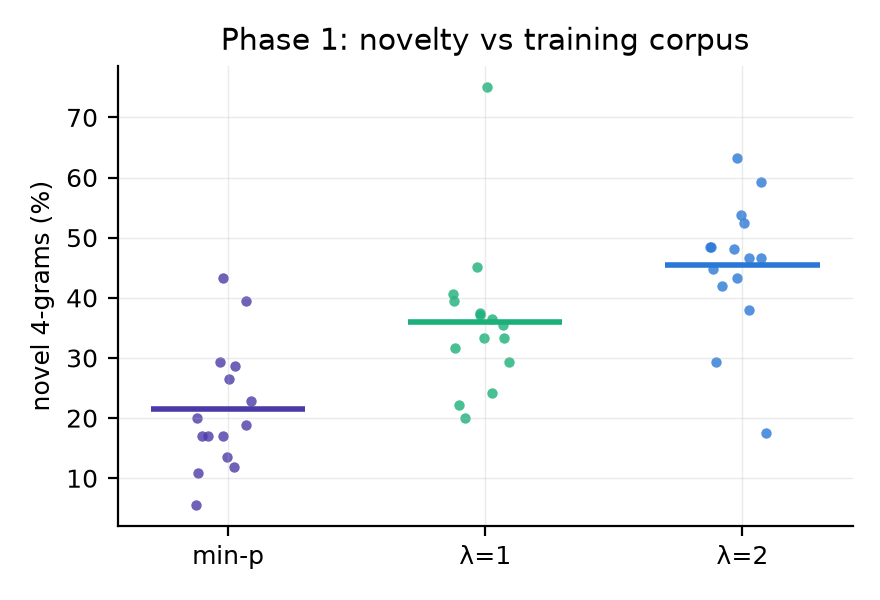
\includegraphics[width=0.72\linewidth]{fig6_phase1_novelty.png}
\caption{Objective novelty against the OLMo-2 training corpus: novel 4-grams
per cell, 3 prompts $\times$ 5 seeds. The anti-probable push roughly doubles
surface novelty over min-$p$ sampling.}
\label{fig:phase1}
\end{figure}

\paragraph{Does it climb?} Two tests say no. In verified search (online bin
packing, the FunSearch benchmark, with a deterministic verifier in place of a
judge; evolutionary loops of 5 runs $\times$ 8 generations $\times$ 20--40
candidates on Qwen3-8B and Qwen3-30B-A3B, 3,200 verified heuristics on the
larger model) the anti-probable operator does not separate from plain
sampling: both arms rediscover best-fit at will and neither beats it on held-out
instances. And inside the reverie loop (Section~\ref{sec:loop}), the same
push, against plain sampling in the same scaffold, yields no measurable
difference in judged surprise, connection or novel delta across 1,335
judgments by two judges under three rubrics (the surprise rubric: 2.97 vs
3.48, CI of the difference \ci{-1.50}{+0.49}). Surface novelty is real, and it
does not rise to the level of ideas.

\section{Hypothesis 2: the prompt}
\label{sec:prompt}

We composed three kinds of input (a typical request, a distant concept pair
drawn from a band of embedding distances, and a composed improbable
context) plus two ablations (fragments only, register only), had Claude
Opus~5 develop each into an idea, and had Claude Sonnet~5 judge the result
against its nearest known equivalent ($k=3$; $n\approx15$ per arm). Input
improbability was measured two ways: semantic $k$NN distance to 10,000 real
prompts (all-mpnet-base-v2) and perplexity. The typical prompt matched or beat
every improbable arm, two of which were significantly worse; improbability
did not correlate with judged novelty ($|r|<0.2$, Figure~\ref{fig:prompt});
a pilot effect ($n=8$) had not replicated. Improbable inputs from outside are
noise, at least when a strong model develops them and a strong model judges.

\begin{figure}[t]
\centering
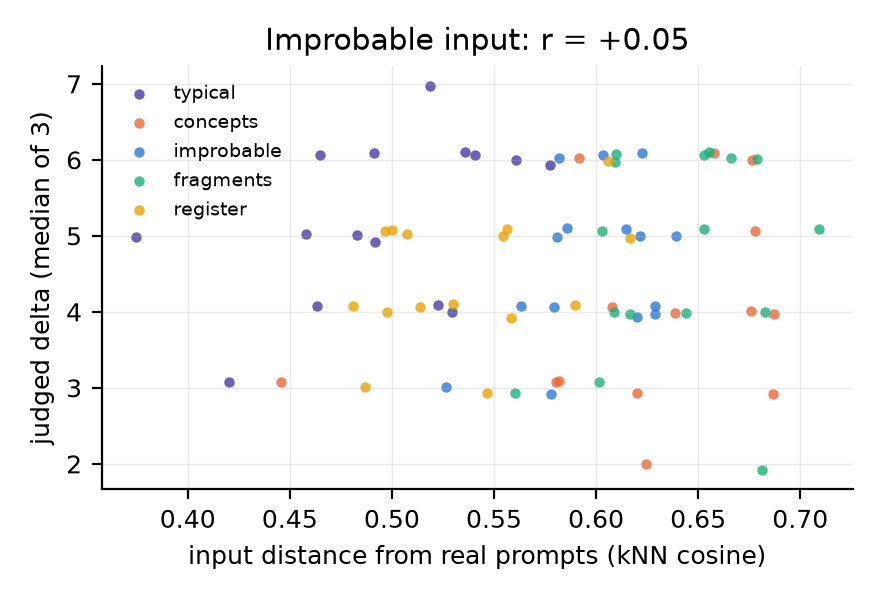
\includegraphics[width=0.72\linewidth]{fig7_improbable_input.png}
\caption{Judged novel delta of the developed idea against the input's
semantic distance from 10,000 real prompts, per arm. No relationship.}
\label{fig:prompt}
\end{figure}

\section{Hypothesis 3: the loop}
\label{sec:loop}

All results in this section use Qwen3-30B-A3B-Base unless stated, ten
narrative seeds, 4,500 tokens per cell, $\lambda=0$, and Claude Opus~5 as
judge with $k=5$. Full tables, including Cliff's $\delta$, Mann--Whitney
$p$-values and paired-by-seed intervals, are in Appendix~\ref{app:loop}.

\subsection{Bare generation is dead; the loop brings it to life}

Left to continue a premise with nothing else, the base model converges within
a few hundred tokens on an attractor of its pretraining and stays there:
\emph{``Highly recommended. Highly recommended.\,\ldots''} for two thousand
tokens; a table of three-digit numbers; an English-exam answer key. Judged
surprise 0.28, connection 0.20, coherence 2.06 (50 windows). The full scaffold
brings the stream to 3.19 / 1.64 / 3.68 (Cliff's $\delta=+0.88$ vs bare on
surprise, $p\approx5\times10^{-15}$; every seed moves in the same direction,
Figure~\ref{fig:perseed}), and elaborates its own finds after a
re-encounter (\emph{``Everything that almost happened piled up inside her like
snow falling sideways through open windowsills into rooms filled with silence
instead of noise\,\ldots\ She kept a notebook because sometimes almosts piled
up too much to be ignored''}). Salience-gated review also beats reviewing on a
timer as a policy for \emph{which} windows to judge (surprise and connection
CIs positive at a third of the judge cost).

\begin{figure}[t]
\centering
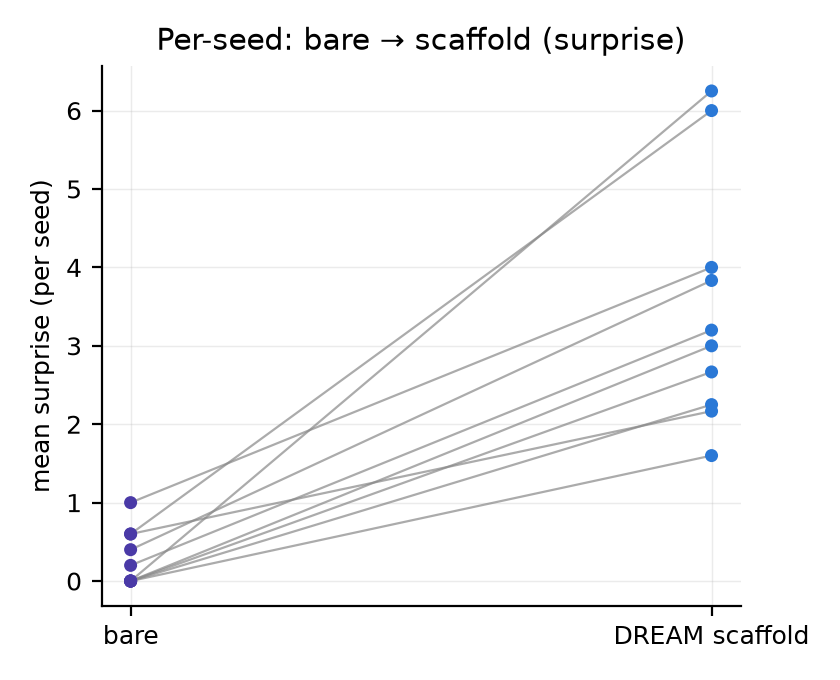
\includegraphics[width=0.6\linewidth]{fig3_per_seed_scaffold_vs_bare.png}
\caption{Per-seed robustness: mean surprise of bare vs scaffold windows, one
line per seed.}
\label{fig:perseed}
\end{figure}

\subsection{Taking the loop apart}
\label{sec:ablation}

Ablation over 10 seeds (Figure~\ref{fig:ablation}, Table~\ref{tab:ladder})
gave the first surprise: \emph{bare + clock reseed} (no salience, no
forgetting, no kicks, only a neutral subject change every 150 tokens over the
preserved context) ties the full scaffold on surprise (3.08 vs 3.19, CI
\ci{-0.54}{+0.78}) and beats it on connection (3.15 vs 1.64, $\delta=-0.58$
for the scaffold, $p\approx1.5\times10^{-7}$) and coherence (4.78 vs 3.68), with
12/60 windows judged both surprising and coherent against 8/47 for the
scaffold and 0/50 for bare. Salience-only (review windows marked but nothing
injected) reaches 2.63. In sentence-embedding space
(Figure~\ref{fig:traj}) bare generation has explored radius 0.18 and mean step
0.14 and ends 0.78 from the premise; the scaffold has radius 0.51 and returns
to within 0.57 of the premise; the clock reseed spreads over the space in
jumps while keeping the whole context, which is where its connection
advantage comes from.

\begin{figure}[t]
\centering

\includegraphics[width=\linewidth]{fig1_reverie_distributions.png}
\caption{Ablation: judged surprise, connection and coherence by arm (10
seeds, Opus~5, median of $k=5$ per window; violins are distributions, bars are
means with bootstrap CIs). Bare + clock reseed matches the full scaffold on
surprise and exceeds it on connection and coherence.}
\label{fig:ablation}
\end{figure}

\begin{figure}[t]
\centering
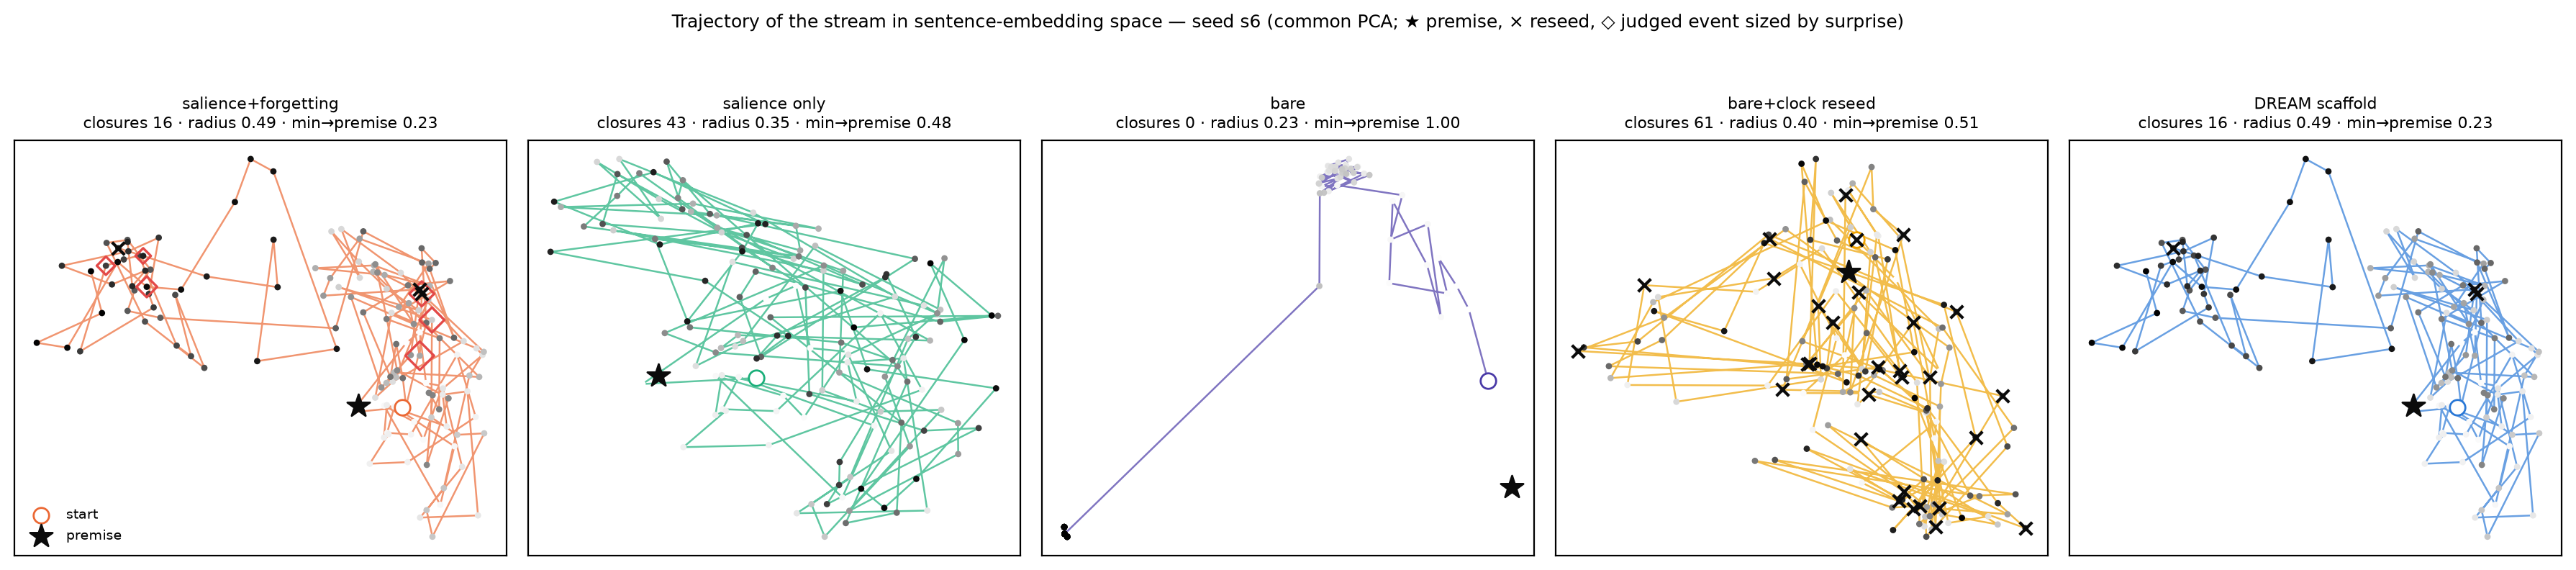
\includegraphics[width=\linewidth]{traj_dream_scaffold_s6.png}
\caption{Where the stream goes: trajectories in sentence-embedding space
(64-token windows, one PCA per seed), seed 6. $\star$ premise, $\circ$ start,
$\times$ reseed, $\diamond$ judged event sized by surprise. Bare makes one
jump and freezes; the scaffold orbits and returns; the clock reseed jumps
across the space keeping its context.}
\label{fig:traj}
\end{figure}

\subsection{What the interruption is made of}
\label{sec:battery2}

The ablation left the effect in one operation and raised four questions about
it, and one about itself. Battery 2 answers them (Table~\ref{tab:ladder},
Figures~\ref{fig:q1}--\ref{fig:q4}).

\paragraph{A confound, and two operations.} The bare arm of the ablation ran
without the scaffold's habituation penalty, which every interrupted arm had;
bare generation dies in \emph{literal} orbits, precisely what a repetition
penalty undoes. Adding the missing control (habituation, no interruption)
splits the effect in two: bare 0.28 $\rightarrow$ bare + habituation
\textbf{1.70} (surprise $\Delta$ +1.42 \ci{+1.12}{+1.72} paired by seed;
connection 0.20 $\rightarrow$ 1.08; coherence 2.06 $\rightarrow$ 4.08)
$\rightarrow$ bare + habituation + clock reseed \textbf{3.08} ($\Delta$ +1.38
\ci{+0.92}{+1.92}). Habituation removes the literal orbits and buys about
half of the surprise; the interruption buys the other half and \emph{all} of
the connection (1.08 $\rightarrow$ 3.15, $\Delta$ +2.07 \ci{+1.63}{+2.57},
$\delta=+0.75$) and the coherence. The full scaffold adds surprise +1.49
\ci{+0.80}{+2.19} over habituation alone but only +0.55 of connection.

\begin{table}[t]
\centering\small
\begin{tabular}{@{}lccc@{\hspace{1.2em}}ccc@{\hspace{1.2em}}ccc@{}}
\toprule
& \multicolumn{3}{c}{Qwen3-30B-A3B} & \multicolumn{3}{c}{Qwen3-8B} & \multicolumn{3}{c}{OLMo-2-13B} \\
\cmidrule(lr){2-4}\cmidrule(lr){5-7}\cmidrule(lr){8-10}
arm & S & C & H & S & C & H & S & C & H \\
\midrule
bare & 0.28 & 0.20 & 2.06 & 0.68 & 0.38 & 3.45 & 1.35 & 0.91 & 2.97 \\
bare + habituation & 1.70 & 1.08 & 4.08 & 1.47 & 0.87 & 3.93 & 2.37 & 1.51 & 4.05 \\
bare + habituation + clock reseed & \textbf{3.08} & \textbf{3.15} & \textbf{4.78} & \textbf{2.73} & \textbf{3.23} & 4.42 & \textbf{3.11} & \textbf{3.17} & 3.28 \\
DREAM scaffold & 3.19 & 1.64 & 3.68 & 2.73 & 1.53 & 4.30 & 3.08 & 1.89 & \textbf{4.48} \\
\bottomrule
\end{tabular}
\caption{The ladder on three generator families: judged surprise (S),
connection (C) and coherence (H), means over windows (Opus~5, $k=5$; 10 seeds
per arm; windows before 100 generated tokens excluded). Habituation buys part
of the surprise; the interruption buys the rest and all of the connection; the
scaffold adds nothing over the plain interruption except, on OLMo, coherence
(its selective forgetting lifts the stream out of a web-boilerplate well).}
\label{tab:ladder}
\end{table}

\begin{figure}[t]
\centering
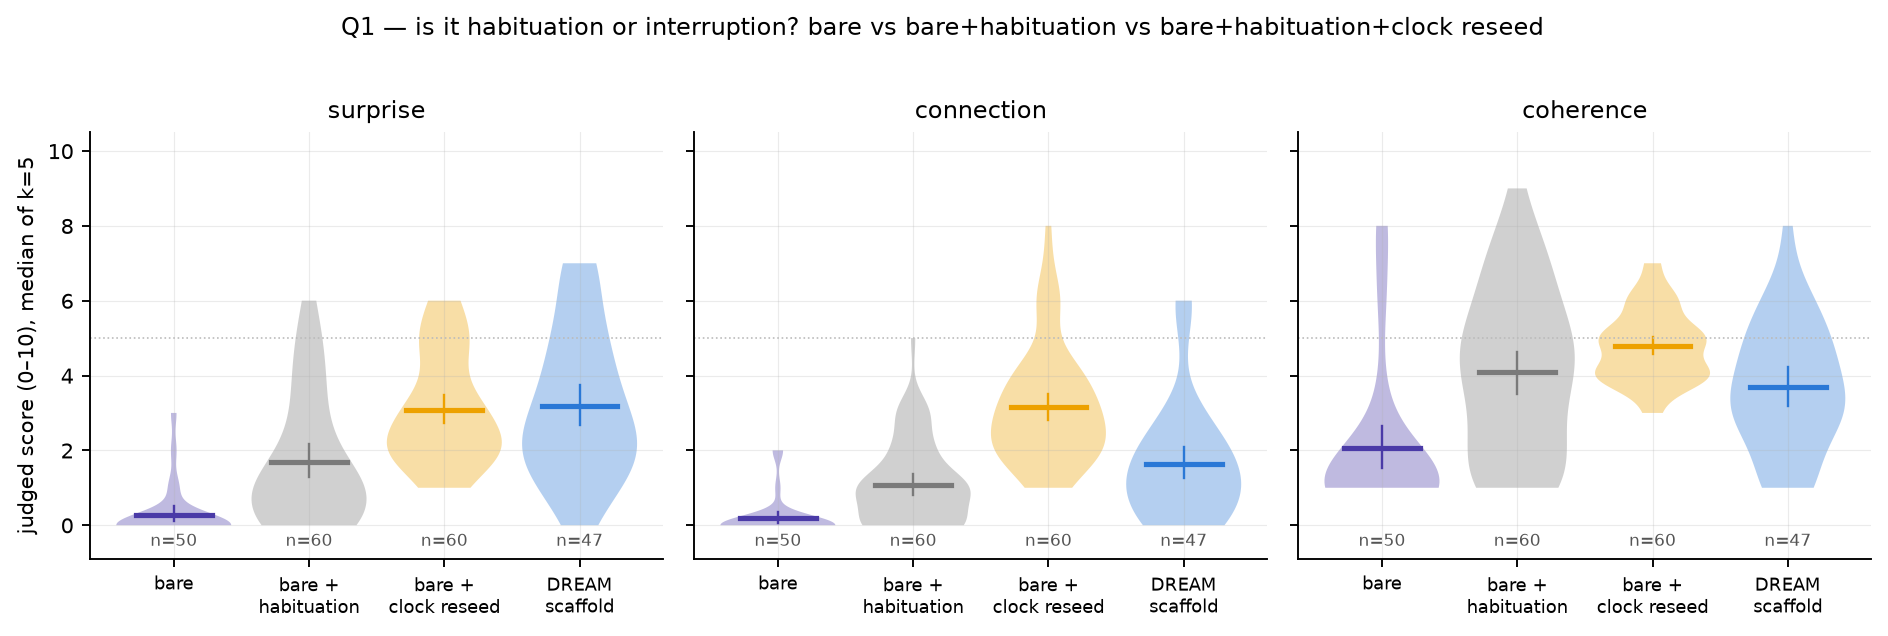
\includegraphics[width=\linewidth]{fig8_q1_habituation.png}
\caption{Habituation or interruption? bare $\rightarrow$ bare + habituation
$\rightarrow$ bare + habituation + clock reseed $\rightarrow$ scaffold
(Qwen3-30B-A3B).}
\label{fig:q1}
\end{figure}

\paragraph{The interruption must lead away.} With the same period (150), a
neutral subject change and a re-encounter stitch that asks the stream to
return to its beginning are close (3.08 / 3.15 / 4.78 vs 2.68 / 3.64 / 4.72;
the stitch trades some surprise for connection, not significantly). Injecting
the \emph{premise itself} (1.14 / 1.04 / 3.18) or a window of the stream's
\emph{own past} (1.42 / 1.52 / 3.06) is as bad as not interrupting at all:
every paired CI against the neutral change excludes zero (connection $-2.11$
\ci{-2.83}{-1.46} and $-1.63$ \ci{-2.37}{-0.91}; $\delta\approx-0.6$ to
$-0.7$). Qualitatively, the own-past injection reinforces whatever attractor
the stream is in: an exam-key well was fed its own questions back. A return
works only as a short stitch that still opens a new sentence; a literal return
closes the loop (Figure~\ref{fig:q2}).

\begin{figure}[t]
\centering

\includegraphics[width=\linewidth]{fig8_q2_content.png}
\caption{Content of the interruption at period 150: neutral change,
re-encounter stitch, the premise itself, the stream's own past. Injecting a
return is as bad as not interrupting.}
\label{fig:q2}
\end{figure}

\paragraph{Salience is a good reader and a bad metronome.} The stitch
injected on salience events (jump, crystallization, recurrence; 1--9 per cell,
median $\approx$5) makes the \emph{event windows} better than salience-only
(3.92 / 2.99 / 3.75 vs 2.63 / 1.39 / 3.71), but the \emph{stream} it produces
is poor: uniform windows 2.18 / 1.68 / 3.93 against \textbf{4.70 / 3.48 /
5.50} for the same stitch on a clock of matched frequency (every 900 tokens;
surprise $\Delta$ +2.02 \ci{+1.62}{+2.44} paired, coherence +0.78) and 5.48 /
2.87 / 5.95 for a neutral change every 900 (45/60 windows both surprising and
coherent, the best cell of the program). Salience events select good moments
to look at, which is why salience-gated review beat clock review; as an
interruption trigger they fire rarely and unevenly and leave streams stuck for
thousands of tokens. Salience should decide where to look, not when to
interrupt (Figure~\ref{fig:q3}).

\begin{figure}[t]
\centering

\includegraphics[width=\linewidth]{fig8_q3_timing.png}
\caption{When to return: the re-encounter stitch on the clock (150 and 900),
on salience events, and salience-only; event windows and uniform windows.}
\label{fig:q3}
\end{figure}

\paragraph{The yield of an interruption depends on the thread it breaks, and
decays with distance from it.} With the neutral change every 75 tokens the
stream is dead (0.88, $\delta=-0.83$ vs 150): nothing has time to develop.
Every 150: 3.08. Every 300, 600 and 900, the windows that end within
$\approx$160 tokens after an interruption score \textbf{5.28 / 3.35 / 5.95},
5.40 / 3.20 / 5.65 and 5.90 / 2.80 / 6.10, the highest values in the
program (34/60 of the 300-early windows both surprising and coherent), while
windows deeper into a segment fall back to $\approx$3.2 and stay there. The
same window shape (a break plus 150 tokens of development) scores 3.08 when
the broken thread was 150 tokens long and 5.3--5.9 when it was 300--900:
surprise needs a developed background to break. Weighting the two phases by
their share of the stream, period 300 gives the best stream (4.35 / 3.18 /
5.97), then 600 (3.82), 900 (3.68), 150 (3.08) and 75 (0.88); connection
falls as segments lengthen (Figure~\ref{fig:q4}). The loop's rhythm is: let a
thread develop for a few hundred tokens, then break it away.

\begin{figure}[t]
\centering

\includegraphics[width=\linewidth]{fig8_q4b_phase.png}
\caption{How often to interrupt. Left: judged surprise against tokens since
the last interruption, per period. Right: stream mean by period. Surprise
peaks in the 150 tokens after a break and decays; a break every 75 tokens
develops nothing.}
\label{fig:q4}
\end{figure}

\subsection{Three generator families}
\label{sec:families}

The ladder replicates on Qwen3-8B-Base and OLMo-2-13B (Table~\ref{tab:ladder},
Figures~\ref{fig:fam8b}--\ref{fig:famolmo}). On the 8B: 0.68 $\rightarrow$
1.47 $\rightarrow$ 2.73 (connection 0.87 $\rightarrow$ 3.23, $\delta=+0.80$),
scaffold 2.73 / 1.53. On OLMo, whose bare stream wanders across web genres
rather than locking into literal orbits and is therefore less dead
(1.35), the same ordering holds on surprise and connection (2.37
$\rightarrow$ 3.11; connection 1.51 $\rightarrow$ 3.17, $\delta=+0.58$), with
one new nuance: the plain interruption \emph{costs} coherence there ($-0.77$
\ci{-1.58}{+0.03}; the injected narrative seed lands on 4,000 tokens of
footers) and the scaffold's selective forgetting is what preserves it (4.48
vs 3.28), the mechanism the calibration probes had suggested. Whether
forgetting is worth its connection cost depends on how deep the generator's
well is.

\begin{figure}[t]
\centering

\includegraphics[width=\linewidth]{fig8_q5_family8b.png}
\caption{The ladder on Qwen3-8B-Base.}
\label{fig:fam8b}
\end{figure}
\begin{figure}[t]
\centering
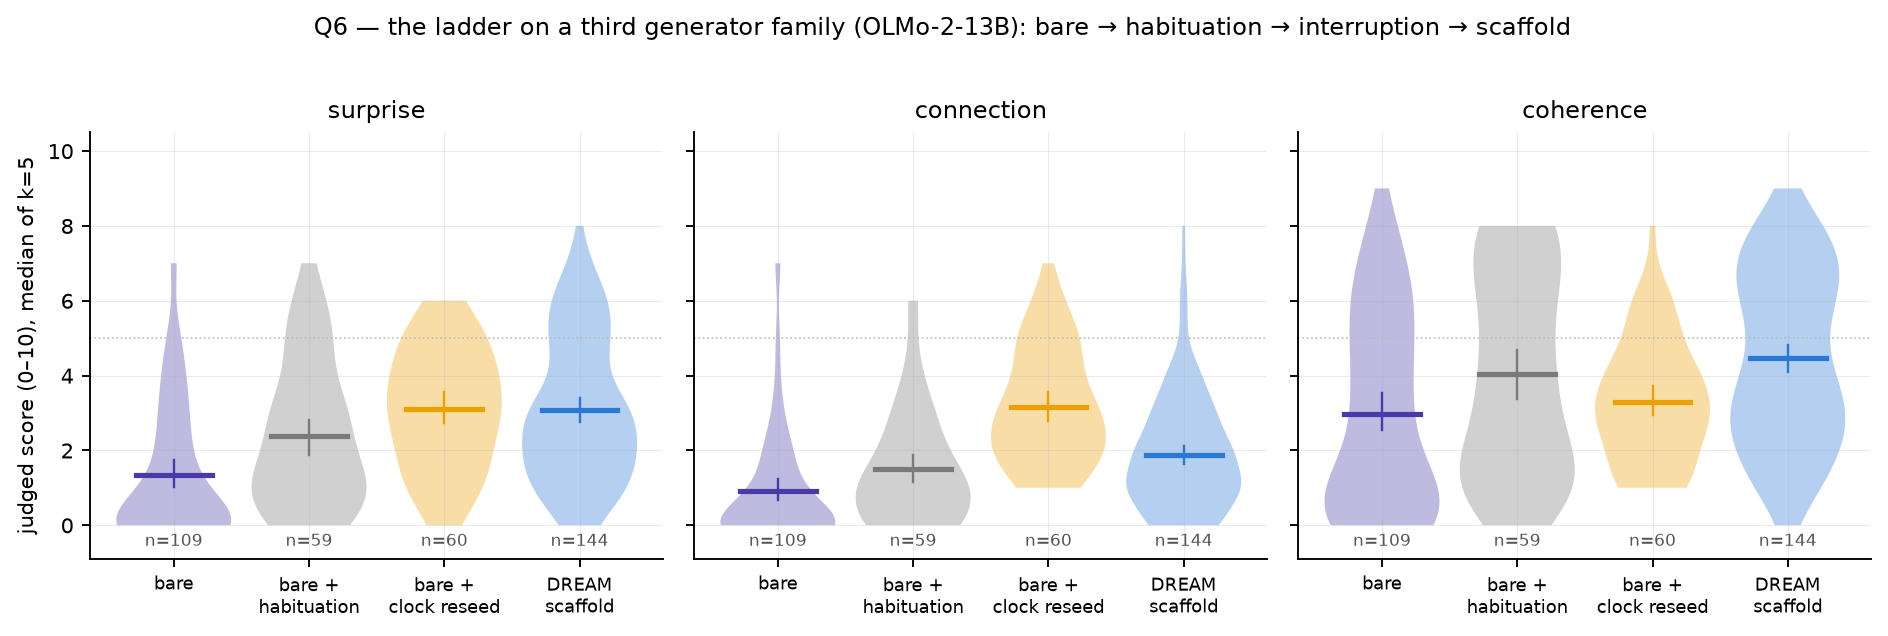
\includegraphics[width=\linewidth]{fig8_q6_familyolmo.png}
\caption{The ladder on OLMo-2-13B: same ordering; the plain interruption
costs coherence and forgetting preserves it.}
\label{fig:famolmo}
\end{figure}


\section{Inside the network: a descriptive look}
\label{sec:network}

Judges and sentence embeddings see the text; the model's own residual stream
sees the computation. This section is exploratory and descriptive: it reports
correlational geometry of the residual stream with judged windows as
observations (clustered by cell; for the pooled correlations we give
cluster-robust intervals from a bootstrap over cells, and the within-condition
values are descriptive), uses a logit lens for one coarse quantity,
and makes no causal intervention. It characterizes what the judged dimensions
co-vary with in the model's state; it does not establish a mechanism. We re-run every finished stream through its generator
(one forward pass with a KV cache, exact token positions) and capture the
residual at 13 layers (every 4th of 48 for Qwen3-30B-A3B; every 3rd for the
36-layer Qwen3-8B and the 40-layer OLMo-2), mean-pooled over 64-token windows
(stride 32) and mean-centered per layer before cosine geometry, plus a logit
lens at each captured layer (the final norm and unembedding applied to the
intermediate state). Three questions.

\paragraph{N1: where does the stream freeze?} Per-layer trajectory
geometry of the window vectors (mean step between consecutive windows,
explored radius) by condition, and the logit-lens \emph{commitment
layer}, the captured layer from which the top-1 token no longer changes.
Bare generation's mean step is a third to a quarter of every interrupted
condition's at every sampled layer; its explored radius is 0.13 at the input layers
against 0.42--0.53, and the gap narrows with depth but never closes (0.24 vs
0.33--0.34 at layer 47, CIs disjoint; Figure~\ref{fig:n1}). The three
interrupted conditions are geometrically alike inside the network; what
separates them is what the judge reads. On the 30B, bare generation's top-1
stabilizes \emph{later} (commitment index 11.12 \ci{11.04}{11.25} of 12 vs
10.88--10.96) while its final distribution is far more confident (final
entropy 0.34 vs 0.42--1.08), a pattern consistent with copying, a late-layer
computation that ends certain; the ordering does not replicate on the 8B, so
we report it as an observation. The 8B and OLMo replicate the geometry (bare
radius 0.14 and 0.36 at layer 0 against 0.46--0.61).

\begin{figure}[t]
\centering
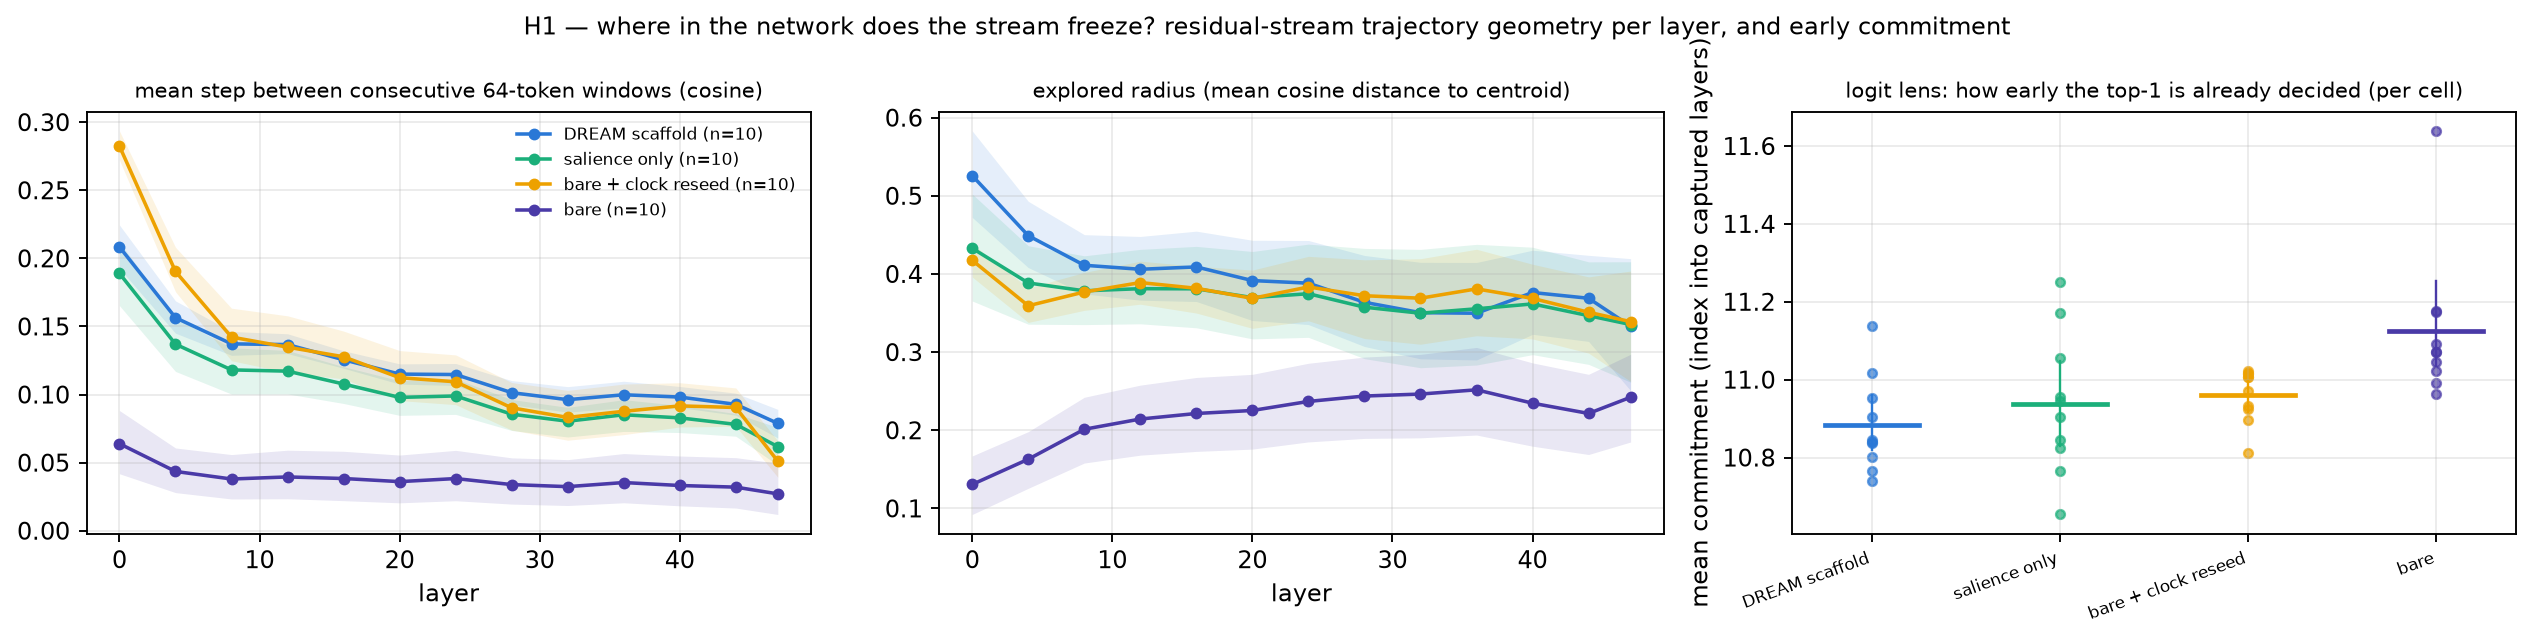
\includegraphics[width=\linewidth]{hidden_h1_geometry_scaffold.png}
\caption{N1: residual-stream trajectory geometry per layer and condition
(Qwen3-30B-A3B, ablation battery): mean step, explored radius, and logit-lens
commitment. Bare generation moves least at every sampled layer, most so at the surface.}
\label{fig:n1}
\end{figure}

\paragraph{N2: which layer's movement predicts judged surprise?} For
every judged window, its novelty at layer $l$ (cosine distance between the
window's mean state and the mean state of everything before it) and its local
step (vs the previous 160 tokens), correlated with judged surprise
(Figure~\ref{fig:n2}). Pooled over conditions, novelty against the past
correlates with surprise at the input layers ($\rho=+0.47$ at layer 0;
cell-bootstrap 95\% CI \ci{+0.22}{+0.67}) and not at the top ($-0.04$,
\ci{-0.26}{+0.17}), but the pooled number is carried by the
bare/interrupted contrast. Within interrupted conditions the sign flips with
depth: local step at layer 0 correlates positively with surprise
(salience-only $+0.46$, scaffold $+0.23$) and at layer 47 negatively
($-0.34$, $-0.14$); novelty against the whole past is negative at depth
(salience-only $-0.53$ at layer 47). Across the 668 judged windows of
battery~2, layer-0 movement predicts surprise within every condition
($\rho$ +0.3 to +0.6), and higher final entropy predicts it everywhere
($\rho$ +0.3 to +0.6): confident is unsurprising. In these data, judged
surprise co-varies with departure at the surface layers and with continuity
at depth: new at the surface, continuous underneath.

\begin{figure}[t]
\centering
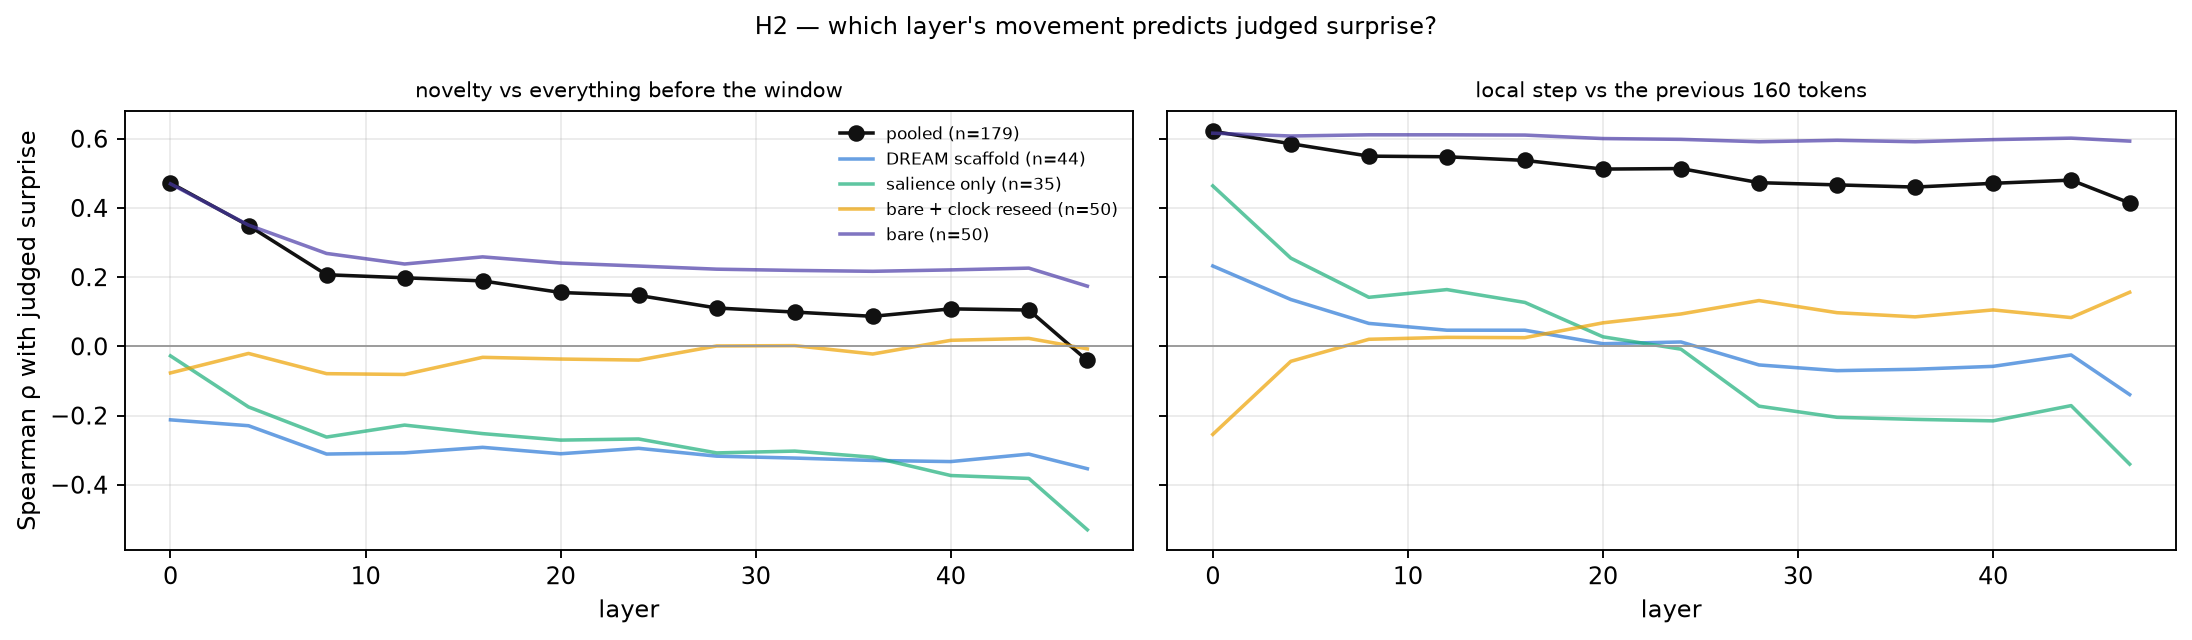
\includegraphics[width=\linewidth]{hidden_h2_novelty_scaffold.png}
\caption{N2: Spearman correlation between the judged window's movement
(novelty vs everything before it, left; local step, right) at each layer and
judged surprise, pooled and within condition.}
\label{fig:n2}
\end{figure}

\paragraph{N3: how deep does an interruption reach?} Cosine distance
between the 64 tokens before an injection and the 64 after it (the injected
text skipped), per layer, minus the same at random positions; and the change
in similarity to the premise's own state (Figure~\ref{fig:n3}). Across a
scaffold reseed \emph{with forgetting}, the state after the injection differs
from the state before by +0.09 (layer 4) growing to +0.21 (layer 40) beyond
control, and its similarity to the premise's state rises by +0.09 to +0.20
with depth: forgetting moves the deep state toward the premise's own state,
a re-encounter with the beginning as the network represents it. Across a clock reseed \emph{over preserved
context} the same measures are +0.01--0.03 and $\approx$0 at every
layer, and this is the interruption the judge rewards most. In this reading,
judged surprise and connection do not track deep representational shifts;
they accompany surface departures over a deep state that is left nearly
intact. We take this as a description of what the judged dimensions track,
not as an account of why the arm scores as it does. The dissociation replicates on the 8B (+0.03 to +0.10 vs
+0.01--0.03) and, larger, on OLMo (+0.20 to +0.38 with a return of +0.13 to
+0.18, vs +0.02--0.06 with no return). In battery 2, the depth of the state
change scales with the length of the interrupted segment (period 75:
$\approx$0; 150: +0.01--0.02; 300: +0.02--0.04; 600: +0.04--0.075) and not
with what is injected (the internal counterpart of the frequency result), and
the salience-timed stitch is the one 150-scale injection that reliably moves
the deep state and pulls it toward the premise, while being the arm whose
stream the judge rates lowest: deep movement and judged quality dissociate
here too. Along the stream, similarity to the premise state is U-shaped in
depth ($\approx$0.9 at layer 0, $\approx$0.5 mid-network, rising at the top)
and ordered at the top layer scaffold 0.85 $>$ salience-only 0.79 $>$ clock
reseed 0.67 $>$ bare 0.55: the sentence-embedding ``return to the premise'' of
the scaffold is visible at the top layer and not in the middle of the network.

\begin{figure}[t]
\centering
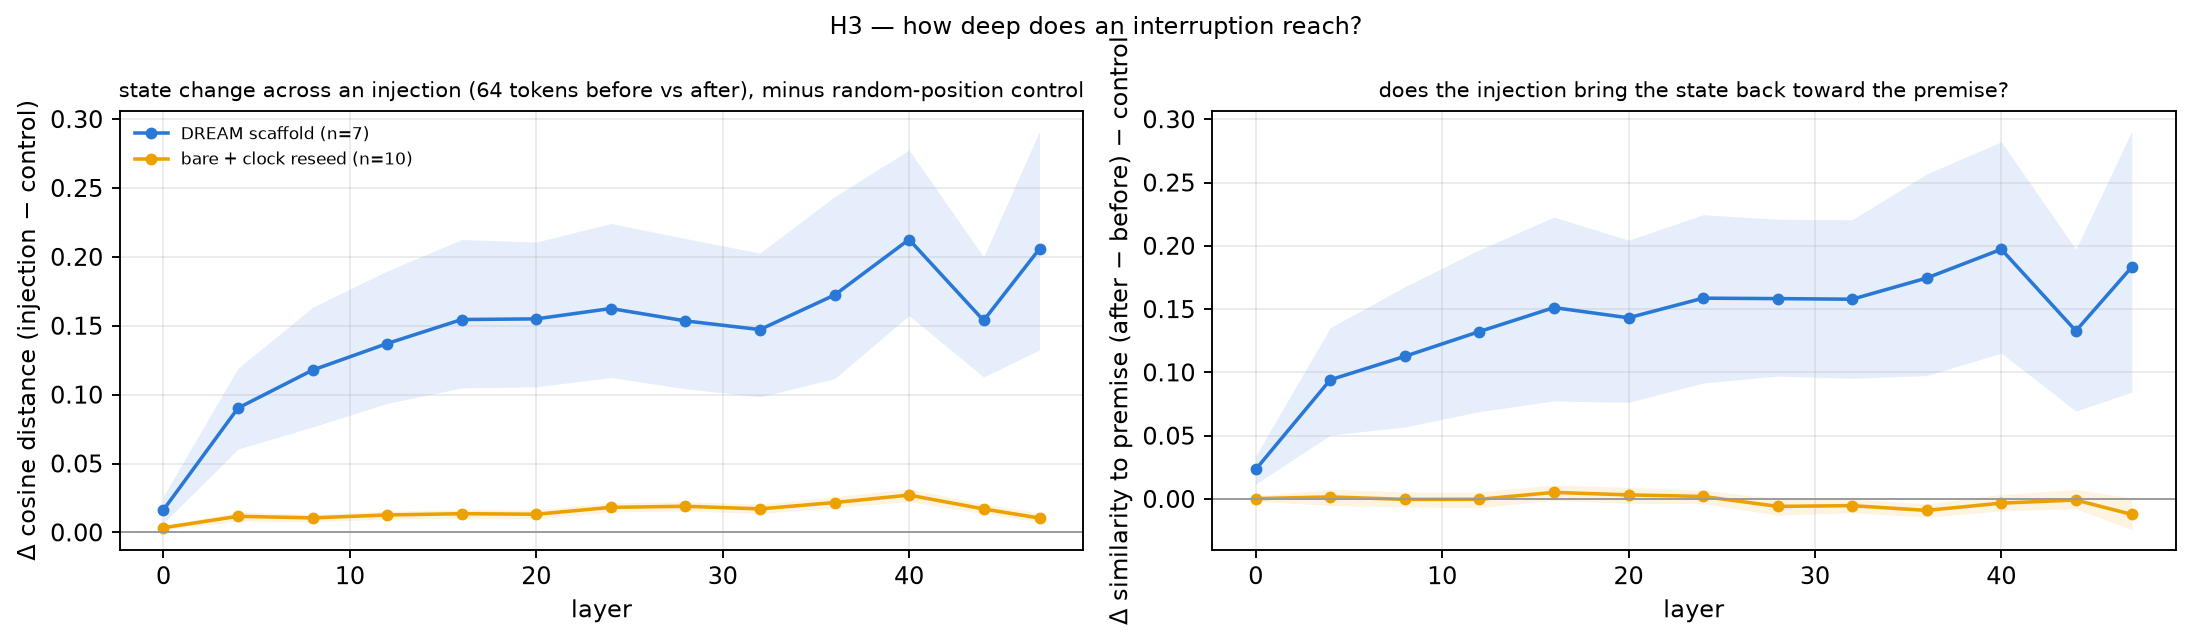
\includegraphics[width=\linewidth]{hidden_h3_interruption_scaffold.png}
\caption{N3: how deep an interruption reaches (Qwen3-30B-A3B). Left: state
change across an injection per layer, minus random-position control. Right:
change in similarity to the premise's own state. The forgetting reseed moves
the deep state and returns it toward the premise; the clock reseed over
preserved context barely touches it, and is what the judge rewards.}
\label{fig:n3}
\end{figure}

\section{The instrument, measured}
\label{sec:instrument}

Every idea-level claim in this paper rests on an LLM judge, so we measured the
judge before using it. On the same 89 windows judged $k=5$ times by two
models, Claude Opus~5 gives continuous scores with an intra-window spread of
0.71 (resolution at about $\pm0.7$); Claude Sonnet~5 has spread 0.27, but by
scoring zero on the connection dimension almost everywhere---a ruler that only
reads ``0'' is consistent (Figure~\ref{fig:judge}). The three-dimension
surprise/connection/coherence rubric has spreads of 0.45--0.70 under Opus.
The consequences shape the paper: LLM judges detect effects of one to two
points (scaffold vs bare, salience vs clock, habituation vs interruption) and
cannot adjudicate half-point effects (push vs plain), which is why the
sampler's null inside the loop is reported as ``undetectable at this
resolution'', not ``absent''; and a binary threshold on a noisy judge is a
coin---the same window scored 5.24 one night and 4.48 the next---so every
result here uses continuous medians of $k$ samples.

\begin{figure}[t]
\centering
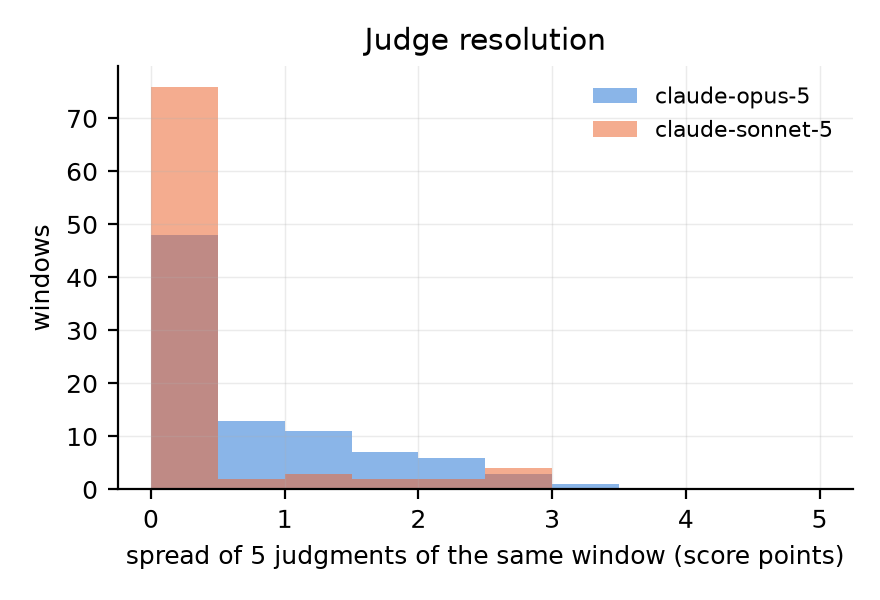
\includegraphics[width=0.7\linewidth]{fig5_judge_resolution.png}
\caption{Spread of five judgments of the same window (delta rubric, 89
windows). Sonnet~5 concentrates at zero spread by scoring zero; Opus~5 gives
continuous scores at $\pm0.7$ noise.}
\label{fig:judge}
\end{figure}

\paragraph{A second judge family.} To check that the loop results are not
the taste of one model family, a stratified sample of 140 already-judged
windows (20 per condition across bare, habituation, clock reseed, scaffold,
re-encounter stitch, period 300 and salience-timed re-encounter) was re-judged
by Kimi K2.6 (Moonshot, via OpenRouter) with the same rubric and $k=5$.
Agreement with Opus~5 on the median of five: surprise Spearman $\rho=+0.85$,
connection $+0.77$, coherence $+0.71$ ($n=140$, $p<10^{-22}$). Kimi is more
generous (means about one point higher) and noisier (intra-window spread
2.0--2.6), but every condition ordering replicates---bare 0.55 $\rightarrow$
habituation 3.15 $\rightarrow$ clock reseed 4.30 $\approx$ scaffold 4.10
$\rightarrow$ period 300 5.65 on surprise, and the neutral reseed and the
re-encounter stitch highest on connection under both judges.

\paragraph{Human rating.} A blind rating of 63 windows (nine per condition,
stratified by judged surprise, shuffled, no labels, the earlier text shown) by
two independent raters, native English readers hired without knowledge of the
hypotheses and instructed not to use AI tools, is in progress; we will report
inter-rater agreement (Krippendorff's $\alpha$) and human--judge Spearman
correlation per dimension. \todo{fill in when the ratings arrive}

\section{Discussion}
\label{sec:discussion}

\paragraph{The scaffold and the beam.} We started from an architecture
modeled on the mind (three networks, incubation, re-encounter), and
measurement returned something simpler and stronger than the architecture.
The DREAM scaffold works, but when it is taken apart almost all of its effect
lives in two operations that were not the noble ones: not eating one's literal
past, and being made, every few hundred tokens, to start a new sentence
somewhere else while remembering everything. We call this minimal recipe the
\emph{interrupted loop}. The elaborate parts either add
nothing (kicks, escalation), or cost something (forgetting costs connection),
or work opposite to their design (a literal return to the premise closes the
loop; salience is a good reader of the stream and a bad metronome for it).
Only because the whole scaffold was built and then dismantled do we know which
beam carries the weight, and which pieces are conditional: forgetting earns
its keep on a generator whose well is web boilerplate, and not on one that
drifts in prose.

\paragraph{Surface novelty and idea novelty are different quantities.} The
anti-probable sampler doubles $n$-gram novelty against the training corpus and
does nothing to judged surprise or connection; the interruption does nothing
special to $n$-grams and lifts judged surprise from 0.3 to 3--6. Inside the
network the two live at different depths: what the judge calls surprise is
lexical departure over an intact deep context, not a deep representational
shift, and the interruption that works barely moves the deep state. This is
also why the neat expectation ``novelty = distance from what came before''
fails: within interrupted streams, deep departure from the stream's own past
is \emph{negatively} related to judged surprise. The reader rewards the window
that is new on the surface and continuous underneath, which is what a good
turn in a story is.

\paragraph{Rhythm.} The frequency result is, we think, the most usable one:
a stream cut every 75 tokens develops nothing; the same break that scores 3.1
after a 150-token thread scores 5.3--5.9 after a 300--900-token thread; and
the yield decays over the next few hundred tokens. Surprise needs a developed
background to break, and interruption is a resource with a rate. The rhythm
we found, develop for a few hundred tokens and then break away, is the
incubation structure in miniature, the coffee break of a working mind: leave,
and be made to come back on your own.

\paragraph{What this is not.} It is not a claim that these streams are good
literature; most windows are judged well below the midpoint, and the texts are
what an unsupervised base model produces. It is not a claim about scale; the
generators are 8--30B parameters at 8 bits. It is a claim about \emph{where}
the novelty a base model can produce with no task comes from, made with
controls, three generator families and two judge families, and it points at
the loop's rhythm rather than at the two places where effort is usually
spent.

\section{Limitations}
\label{sec:limitations}

\paragraph{What was measured.} The outcome is \emph{judged narrative
surprise, connection and coherence} on short windows of forced open-ended
continuation, read by an LLM judge and, on a subset, by human readers. That
is a defensible operationalization of one ingredient of creativity, the
appropriately unexpected turn. It is not creativity: no value, interest or
originality against the world is measured, and the study makes no claim
about ideas or problems. Its title names the question the program set out
with; the results answer a narrower one.

\paragraph{Design.} The premises are ten English narrative openings, plus
ten expository openings for one replication and ten new narrative premises
for the confirmatory battery. Three generator models from two families run
the core ladder; one generator (Qwen3-30B-A3B) runs the content, timing,
period and control batteries. Every arm ran once per premise with the same
random seed, so the ten cells are the whole sample and a paired comparison
of ten is the strongest inference available. Batteries 1 to 3 are
exploratory. They were designed in sequence, the questions of batteries~2
and~3 were formulated after seeing battery~1 and after an external review,
and the analysis reported here (generated-only windows, cell as unit) was
fixed before battery~3 was generated but after the earlier arms had been
seen under the first protocol. The pre-registered exception is the
replication of Section~\ref{sec:confirm}, run on new premises and a new
random seed with its contrasts written down in advance; the judge-gated arm
and the verifier probe were pre-registered in the same way. Everything else
should be read as a well-controlled exploratory study.

\paragraph{Instrument.} The judge is one model family. It is calibrated for
repeatability and agrees with a second family ($\rho=0.71$--$0.85$ on
windows) and with the consensus of three human readers ($\rho=0.58$ on
surprise, $0.52$ on coherence, on a judge-stratified sample), whose agreement
with each other is low to moderate ($\alpha=0.30$--$0.38$). Human readers
did not rate connection in round~1, and they penalize the fluency cost of a
subject change more than the judge does. The judge sees 600 tokens of
context, so ``connection'' means connection within that horizon. Text that
the stream copies from further back is invisible to it as a copy, and a
fixed rotation of injected sentences produces exactly such copies
(Section~\ref{sec:ablation}). We report fresh-only estimates for that
reason, and a judge with the whole document in view for the same reason.

\paragraph{Baselines and generality.} The bare arm is a deliberately hard
regime (forced continuation with end-of-text masked, no repetition control).
We report it as the floor of the ladder, not as a fair decoding baseline; the
fair comparisons are habituation alone, habituation with a stronger penalty,
EOS allowed, and the sham and reset controls. Stronger decoding baselines
(look-back or contrastive decoding, learned repetition control) were not
tested. Base models were used by a scope decision. The one post-trained
model we ran, in raw continuation, shows the same ladder at a lower level
and says nothing about the dialogue use such models are made for.

\paragraph{The network section.} The residual-stream analysis is
correlational and descriptive: mean-pooled 64-token windows at 13 sampled
layers, a logit lens for a coarse commitment layer, no attention analysis,
no tuned lens, no causal intervention. It characterizes what the judged
dimensions correlate with in the model's state. It does not establish a
mechanism.

\section{Conclusion}

Three findings carry this paper. First, the novelty a base language model
produces with no task comes, in the regime we studied, from the structure of
the loop and from one simple part of it: damp the model's literal repetition
and interrupt it every few hundred tokens with a sentence that leads
somewhere new, and its generated text is judged more surprising and
somewhat more connected, by an LLM judge from another family and by human
readers, on windows that contain none of the injected words and none of the
stream's own earlier text. A pre-registered replication on new premises
confirms the main contrast. The new subject is what does the work, with or
without the earlier text in the model's memory; a boundary alone does
nothing. Neither the sampler, at the resolution we could reach, nor the
prompt, under the operationalizations we tested, does any of this.

Second, the gains do not compose. Read as documents, these streams remain
collections; a Review that decides when not to interrupt does not change
that; and on a problem with a verifier the same interruption multiplies the
valid, distinct candidates a base model writes without improving the best
of them. The interruption is a variation operator. Whether that variation
becomes value inside a selection loop, where a find is kept because it is
worth something, is the question this study leaves open and the next one
asks.

Third, a windowed LLM judge of a long stream misses things that change the
answer. It scores the experimenter's injected sentence as the model's own,
it scores the model's replay of its own earlier segments as surprise and
connection when the source lies beyond its horizon, and it cannot tell a
local gain from a whole. Generated-only windows, fresh-only estimates, a
document-level reading, the premise as the unit and a measured judge are
what it took to see this, and we suspect they are what it takes in general.
What we have characterized is a controllable intervention on forced
open-ended generation and the instrument needed to characterize it honestly.


\paragraph{Acknowledgements and tooling.} The experiments, analyses and text of this
paper were produced by the author working with Claude (Anthropic) as a
programming and writing assistant inside the Claude Code environment; every
design decision, result and claim was reviewed by the author, and the dated
laboratory notebook, code and per-run data are public in the repository.
Judges were run on Amazon Bedrock and OpenRouter; generators ran locally on
Apple silicon via MLX.

\bibliographystyle{plainnat}
\bibliography{references}

\appendix
\section{Full tables}
\label{app:loop}

The tables below are generated from the run data by the analysis scripts
(\texttt{scripts/analysis.py}, \texttt{analysis\_b2.py},
\texttt{hidden\_analysis.py}) and typeset by \texttt{scripts/appendix\_tex.py};
the complete set, including every per-layer table of the residual-stream
analysis, ships with the code as \texttt{docs/APPENDIX\_*.md}. Unless stated,
the unit is the judged window (median of $k=5$ Opus~5 judgments), windows
before 100 generated tokens are excluded, and intervals are 95\% bootstrap
CIs.

% auto-generated by scripts/appendix_tex.py - do not edit by hand
\subsection*{Generated-only windows, unit = cell (primary analysis)}
\begin{table}[H]
\centering
\scriptsize
\begin{adjustbox}{max width=\textwidth}
\begin{tabular}{@{}lcccc@{}}
\toprule
condition & n cells & surprise & connection & coherence \\
\midrule
bare & 10 & 0.45 [0.28, 0.68] & 0.30 [0.15, 0.45] & 2.52 [1.88, 3.43] \\
bare + habituation & 10 & 1.58 [1.17, 1.98] & 1.28 [0.82, 1.78] & 4.45 [3.47, 5.48] \\
reseed 150, no habituation & 10 & 2.47 [2.17, 2.77] & 3.00 [2.57, 3.42] & 5.38 [4.80, 5.85] \\
habituation + reseed 150 & 10 & 3.02 [2.53, 3.53] & 3.68 [2.92, 4.52] & 6.12 [5.60, 6.57] \\
DREAM scaffold & 10 & 2.70 [2.10, 3.40] & 1.85 [1.42, 2.33] & 6.02 [5.32, 6.73] \\
habituation 1.3 & 10 & 1.77 [1.38, 2.23] & 1.42 [1.05, 1.83] & 4.90 [4.48, 5.38] \\
habituation, EOS allowed & 10 & 1.55 [1.10, 1.97] & 1.28 [0.95, 1.67] & 5.72 [4.83, 6.45] \\
\bottomrule
\end{tabular}
\end{adjustbox}
\caption{Generated-only protocol. Q1: habituation $\times$ interruption (period 150) and baselines: cell means (mean over cells [95\% CI over cells]).}
\label{tab:gen-q1}
\end{table}

\begin{table}[H]
\centering
\scriptsize
\begin{adjustbox}{max width=\textwidth}
\begin{tabular}{@{}p{4.6cm}cccccc@{}}
\toprule
condition & dim & $\Delta$ [CI] & p (perm) & q (BH) & Cliff $\delta$ & n seeds \\
\midrule
bare & surprise & -1.13 [-1.47, -0.72] & 0.004 & 0.023 & -0.80 & 10 \\
bare & connection & -0.98 [-1.48, -0.48] & 0.010 & 0.035 & -0.79 & 10 \\
bare & coherence & -1.93 [-3.35, -0.53] & 0.035 & 0.078 & -0.64 & 10 \\
reseed 150, no habituation & surprise & +0.88 [+0.27, +1.47] & 0.039 & 0.078 & +0.70 & 10 \\
reseed 150, no habituation & connection & +1.72 [+0.88, +2.45] & 0.010 & 0.035 & +0.90 & 10 \\
reseed 150, no habituation & coherence & +0.93 [-0.03, +1.93] & 0.127 & 0.176 & +0.37 & 10 \\
habituation + reseed 150 & surprise & +1.43 [+0.93, +2.05] & 0.002 & 0.018 & +0.85 & 10 \\
habituation + reseed 150 & connection & +2.40 [+1.58, +3.32] & 0.002 & 0.018 & +0.93 & 10 \\
habituation + reseed 150 & coherence & +1.67 [+0.27, +2.88] & 0.051 & 0.083 & +0.57 & 10 \\
DREAM scaffold & surprise & +1.12 [+0.40, +1.92] & 0.023 & 0.070 & +0.64 & 10 \\
DREAM scaffold & connection & +0.57 [+0.17, +1.02] & 0.031 & 0.078 & +0.41 & 10 \\
DREAM scaffold & coherence & +1.57 [+0.15, +2.93] & 0.051 & 0.083 & +0.57 & 10 \\
habituation 1.3 & surprise & +0.18 [-0.22, +0.65] & 0.547 & 0.656 & +0.03 & 10 \\
habituation 1.3 & connection & +0.13 [-0.42, +0.60] & 0.680 & 0.765 & +0.11 & 10 \\
habituation 1.3 & coherence & +0.45 [-0.67, +1.47] & 0.484 & 0.623 & +0.23 & 10 \\
habituation, EOS allowed & surprise & -0.03 [-0.48, +0.42] & 0.953 & 1.000 & +0.08 & 10 \\
habituation, EOS allowed & connection & +0.00 [-0.53, +0.47] & 1.000 & 1.000 & -0.01 & 10 \\
habituation, EOS allowed & coherence & +1.27 [+0.10, +2.28] & 0.064 & 0.097 & +0.48 & 10 \\
\bottomrule
\end{tabular}
\end{adjustbox}
\caption{Generated-only protocol. vs bare + habituation: paired by seed.}
\label{tab:gen-q1-diff}
\end{table}

\begin{table}[H]
\centering
\scriptsize
\begin{adjustbox}{max width=\textwidth}
\begin{tabular}{@{}lcccc@{}}
\toprule
condition & n cells & surprise & connection & coherence \\
\midrule
neutral subject change & 10 & 3.02 [2.53, 3.53] & 3.68 [2.92, 4.52] & 6.12 [5.60, 6.57] \\
re-encounter stitch & 10 & 2.80 [2.08, 3.55] & 3.68 [2.80, 4.60] & 5.50 [4.90, 6.12] \\
the premise itself & 10 & 1.18 [0.88, 1.44] & 1.11 [0.77, 1.43] & 3.92 [3.21, 4.68] \\
the stream's own past & 10 & 1.49 [1.07, 1.96] & 1.43 [0.87, 2.04] & 3.70 [3.05, 4.30] \\
\bottomrule
\end{tabular}
\end{adjustbox}
\caption{Generated-only protocol. Q2: what is injected (period 150): cell means (mean over cells [95\% CI over cells]).}
\label{tab:gen-q2}
\end{table}

\begin{table}[H]
\centering
\scriptsize
\begin{adjustbox}{max width=\textwidth}
\begin{tabular}{@{}p{4.6cm}cccccc@{}}
\toprule
condition & dim & $\Delta$ [CI] & p (perm) & q (BH) & Cliff $\delta$ & n seeds \\
\midrule
re-encounter stitch & surprise & -0.22 [-1.18, +0.67] & 0.691 & 0.778 & -0.15 & 10 \\
re-encounter stitch & connection & +0.00 [-1.35, +1.23] & 1.000 & 1.000 & -0.03 & 10 \\
re-encounter stitch & coherence & -0.62 [-1.48, +0.15] & 0.215 & 0.276 & -0.43 & 10 \\
the premise itself & surprise & -1.84 [-2.37, -1.32] & 0.002 & 0.004 & -1.00 & 10 \\
the premise itself & connection & -2.58 [-3.42, -1.79] & 0.002 & 0.004 & -1.00 & 10 \\
the premise itself & coherence & -2.20 [-3.01, -1.43] & 0.002 & 0.004 & -0.87 & 10 \\
the stream's own past & surprise & -1.52 [-2.15, -0.84] & 0.006 & 0.009 & -0.85 & 10 \\
the stream's own past & connection & -2.26 [-3.29, -1.29] & 0.004 & 0.007 & -0.84 & 10 \\
the stream's own past & coherence & -2.42 [-3.23, -1.63] & 0.002 & 0.004 & -0.95 & 10 \\
\bottomrule
\end{tabular}
\end{adjustbox}
\caption{Generated-only protocol. vs neutral subject change: paired by seed.}
\label{tab:gen-q2-diff}
\end{table}

\begin{table}[H]
\centering
\scriptsize
\begin{adjustbox}{max width=\textwidth}
\begin{tabular}{@{}lcccc@{}}
\toprule
condition & n cells & surprise & connection & coherence \\
\midrule
no interruption & 10 & 1.58 [1.17, 1.98] & 1.28 [0.82, 1.78] & 4.45 [3.47, 5.48] \\
paragraph break (sham) & 10 & 1.42 [1.07, 1.78] & 0.97 [0.65, 1.28] & 4.43 [3.60, 5.23] \\
continuity connective (sham) & 10 & 1.08 [0.68, 1.55] & 0.86 [0.48, 1.32] & 3.51 [2.98, 4.15] \\
subject change, context preserved & 10 & 2.90 [2.45, 3.33] & 2.38 [2.02, 2.77] & 6.40 [6.08, 6.70] \\
subject change, no habituation & 10 & 2.48 [2.08, 2.90] & 1.98 [1.55, 2.57] & 5.50 [4.60, 6.33] \\
subject change, context reset & 10 & 3.72 [3.40, 4.07] & 3.32 [3.03, 3.62] & 6.88 [6.65, 7.13] \\
break, context reset & 10 & 2.03 [1.70, 2.47] & 1.73 [1.50, 1.98] & 5.43 [5.12, 5.83] \\
\bottomrule
\end{tabular}
\end{adjustbox}
\caption{Generated-only protocol. Q3: period 300: what carries the effect (context preserved vs reset; semantic change vs neutral boundary): cell means (mean over cells [95\% CI over cells]).}
\label{tab:gen-q3}
\end{table}

\begin{table}[H]
\centering
\scriptsize
\begin{adjustbox}{max width=\textwidth}
\begin{tabular}{@{}p{4.6cm}cccccc@{}}
\toprule
condition & dim & $\Delta$ [CI] & p (perm) & q (BH) & Cliff $\delta$ & n seeds \\
\midrule
paragraph break (sham) & surprise & -0.17 [-0.68, +0.35] & 0.598 & 0.633 & -0.27 & 10 \\
paragraph break (sham) & connection & -0.32 [-0.80, +0.15] & 0.273 & 0.328 & -0.23 & 10 \\
paragraph break (sham) & coherence & -0.02 [-1.08, +1.20] & 1.000 & 1.000 & -0.02 & 10 \\
continuity connective (sham) & surprise & -0.50 [-1.20, +0.25] & 0.246 & 0.316 & -0.38 & 10 \\
continuity connective (sham) & connection & -0.43 [-1.18, +0.38] & 0.344 & 0.387 & -0.36 & 10 \\
continuity connective (sham) & coherence & -0.94 [-2.35, +0.52] & 0.242 & 0.316 & -0.37 & 10 \\
subject change, context preserved & surprise & +1.32 [+0.68, +1.93] & 0.004 & 0.018 & +0.86 & 10 \\
subject change, context preserved & connection & +1.10 [+0.48, +1.67] & 0.014 & 0.047 & +0.74 & 10 \\
subject change, context preserved & coherence & +1.95 [+0.72, +3.18] & 0.021 & 0.055 & +0.64 & 10 \\
subject change, no habituation & surprise & +0.90 [+0.43, +1.38] & 0.016 & 0.047 & +0.70 & 10 \\
subject change, no habituation & connection & +0.70 [-0.07, +1.53] & 0.148 & 0.297 & +0.51 & 10 \\
subject change, no habituation & coherence & +1.05 [-0.13, +2.38] & 0.168 & 0.302 & +0.30 & 10 \\
subject change, context reset & surprise & +2.13 [+1.70, +2.63] & 0.002 & 0.018 & +1.00 & 10 \\
subject change, context reset & connection & +2.03 [+1.60, +2.42] & 0.002 & 0.018 & +0.93 & 10 \\
subject change, context reset & coherence & +2.43 [+1.50, +3.33] & 0.004 & 0.018 & +0.75 & 10 \\
break, context reset & surprise & +0.45 [-0.12, +1.05] & 0.205 & 0.308 & +0.41 & 10 \\
break, context reset & connection & +0.45 [-0.13, +1.02] & 0.203 & 0.308 & +0.47 & 10 \\
break, context reset & coherence & +0.98 [+0.13, +1.82] & 0.070 & 0.158 & +0.49 & 10 \\
\bottomrule
\end{tabular}
\end{adjustbox}
\caption{Generated-only protocol. vs no interruption: paired by seed.}
\label{tab:gen-q3-diff}
\end{table}

\begin{table}[H]
\centering
\scriptsize
\begin{adjustbox}{max width=\textwidth}
\begin{tabular}{@{}p{4.6cm}ccccc@{}}
\toprule
contrast & dim & $\Delta$ [CI] & p (perm) & Cliff $\delta$ & n \\
\midrule
reset vs preserved (300) & surprise & +0.82 [+0.32, +1.30] & 0.020 & +0.63 & 10 \\
reset vs preserved (300) & connection & +0.93 [+0.53, +1.32] & 0.004 & +0.81 & 10 \\
reset vs preserved (300) & coherence & +0.48 [+0.03, +0.95] & 0.090 & +0.53 & 10 \\
with vs without habituation (300) & surprise & +0.42 [-0.17, +1.07] & 0.277 & +0.33 & 10 \\
with vs without habituation (300) & connection & +0.40 [-0.33, +1.07] & 0.352 & +0.46 & 10 \\
with vs without habituation (300) & coherence & +0.90 [+0.07, +1.82] & 0.117 & +0.33 & 10 \\
with vs without habituation (150) & surprise & +0.55 [-0.12, +1.28] & 0.197 & +0.34 & 10 \\
with vs without habituation (150) & connection & +0.68 [-0.27, +1.67] & 0.232 & +0.23 & 10 \\
with vs without habituation (150) & coherence & +0.73 [-0.00, +1.43] & 0.096 & +0.55 & 10 \\
subject change vs break, both reset (300) & surprise & +1.68 [+1.17, +2.17] & 0.002 & +0.91 & 10 \\
subject change vs break, both reset (300) & connection & +1.58 [+1.20, +2.02] & 0.002 & +1.00 & 10 \\
subject change vs break, both reset (300) & coherence & +1.45 [+1.13, +1.80] & 0.002 & +0.91 & 10 \\
subject change vs break, both preserved (300) & surprise & +1.48 [+0.83, +2.07] & 0.006 & +0.89 & 10 \\
subject change vs break, both preserved (300) & connection & +1.42 [+0.97, +1.95] & 0.002 & +0.93 & 10 \\
subject change vs break, both preserved (300) & coherence & +1.97 [+1.12, +2.87] & 0.004 & +0.84 & 10 \\
\bottomrule
\end{tabular}
\end{adjustbox}
\caption{Generated-only protocol. Q3b: direct paired contrasts among the interruption arms.}
\label{tab:gen-q3b}
\end{table}

\begin{table}[H]
\centering
\scriptsize
\begin{adjustbox}{max width=\textwidth}
\begin{tabular}{@{}lcccc@{}}
\toprule
condition & n cells & surprise & connection & coherence \\
\midrule
stitch on the clock 150 & 10 & 2.80 [2.08, 3.55] & 3.68 [2.80, 4.60] & 5.50 [4.90, 6.12] \\
stitch on the clock 900 & 10 & 3.04 [2.70, 3.42] & 2.73 [2.42, 3.07] & 5.72 [5.30, 6.16] \\
neutral change 900 & 10 & 3.18 [2.72, 3.76] & 2.28 [1.78, 2.84] & 6.76 [6.58, 6.92] \\
stitch on salience events & 10 & 3.04 [2.50, 3.59] & 2.92 [2.33, 3.57] & 5.68 [4.94, 6.45] \\
salience only & 10 & 1.65 [1.23, 2.02] & 1.30 [0.85, 1.77] & 4.63 [3.67, 5.65] \\
\bottomrule
\end{tabular}
\end{adjustbox}
\caption{Generated-only protocol. Q4: timing: salience vs clock (same stitch): cell means (mean over cells [95\% CI over cells]).}
\label{tab:gen-q4}
\end{table}

\begin{table}[H]
\centering
\scriptsize
\begin{adjustbox}{max width=\textwidth}
\begin{tabular}{@{}p{4.6cm}cccccc@{}}
\toprule
condition & dim & $\Delta$ [CI] & p (perm) & q (BH) & Cliff $\delta$ & n seeds \\
\midrule
stitch on the clock 150 & surprise & -0.24 [-0.87, +0.40] & 0.496 & 0.744 & -0.22 & 10 \\
stitch on the clock 150 & connection & +0.95 [+0.17, +1.76] & 0.064 & 0.193 & +0.28 & 10 \\
stitch on the clock 150 & coherence & -0.22 [-0.76, +0.30] & 0.457 & 0.744 & -0.16 & 10 \\
neutral change 900 & surprise & +0.14 [-0.46, +0.82] & 0.764 & 0.916 & +0.04 & 10 \\
neutral change 900 & connection & -0.45 [-1.06, +0.28] & 0.250 & 0.500 & -0.45 & 10 \\
neutral change 900 & coherence & +1.04 [+0.60, +1.44] & 0.008 & 0.031 & +0.82 & 10 \\
stitch on salience events & surprise & +0.00 [-0.73, +0.73] & 1.000 & 1.000 & -0.02 & 10 \\
stitch on salience events & connection & +0.19 [-0.61, +0.91] & 0.652 & 0.870 & +0.13 & 10 \\
stitch on salience events & coherence & -0.04 [-0.72, +0.65] & 0.912 & 0.995 & -0.09 & 10 \\
salience only & surprise & -1.39 [-2.06, -0.83] & 0.002 & 0.023 & -0.92 & 10 \\
salience only & connection & -1.43 [-2.13, -0.72] & 0.006 & 0.031 & -0.86 & 10 \\
salience only & coherence & -1.09 [-2.05, +0.08] & 0.100 & 0.239 & -0.46 & 10 \\
\bottomrule
\end{tabular}
\end{adjustbox}
\caption{Generated-only protocol. vs stitch on the clock 900: paired by seed.}
\label{tab:gen-q4-diff}
\end{table}

\begin{table}[H]
\centering
\scriptsize
\begin{adjustbox}{max width=\textwidth}
\begin{tabular}{@{}lcccc@{}}
\toprule
condition & n cells & surprise & connection & coherence \\
\midrule
stitch on the clock 900 & 10 & 2.08 [1.63, 2.48] & 1.73 [1.40, 2.01] & 4.75 [4.07, 5.39] \\
neutral change 900 & 10 & 2.51 [2.14, 2.83] & 2.01 [1.68, 2.34] & 5.33 [4.74, 5.88] \\
neutral change 600 & 10 & 2.88 [2.40, 3.32] & 2.27 [1.88, 2.65] & 5.50 [4.92, 6.00] \\
stitch on salience events & 10 & 1.85 [1.36, 2.30] & 1.80 [1.17, 2.44] & 4.18 [3.76, 4.58] \\
DREAM scaffold & 7 & 1.64 [1.17, 2.14] & 1.46 [1.05, 1.79] & 5.61 [4.65, 6.44] \\
\bottomrule
\end{tabular}
\end{adjustbox}
\caption{Generated-only protocol. Q4b: deep windows (at least 300 tokens after the last injection): the stream when it is left alone: cell means (mean over cells [95\% CI over cells]).}
\label{tab:gen-q4b}
\end{table}

\begin{table}[H]
\centering
\scriptsize
\begin{adjustbox}{max width=\textwidth}
\begin{tabular}{@{}p{4.6cm}cccccc@{}}
\toprule
condition & dim & $\Delta$ [CI] & p (perm) & q (BH) & Cliff $\delta$ & n seeds \\
\midrule
neutral change 900 & surprise & +0.42 [-0.12, +0.96] & 0.186 & 0.299 & +0.36 & 10 \\
neutral change 900 & connection & +0.28 [-0.15, +0.71] & 0.266 & 0.354 & +0.26 & 10 \\
neutral change 900 & coherence & +0.58 [-0.10, +1.33] & 0.188 & 0.299 & +0.25 & 10 \\
neutral change 600 & surprise & +0.80 [+0.08, +1.48] & 0.074 & 0.299 & +0.61 & 10 \\
neutral change 600 & connection & +0.54 [+0.02, +1.08] & 0.125 & 0.299 & +0.45 & 10 \\
neutral change 600 & coherence & +0.75 [-0.06, +1.59] & 0.141 & 0.299 & +0.38 & 10 \\
stitch on salience events & surprise & -0.23 [-0.76, +0.25] & 0.455 & 0.496 & -0.18 & 10 \\
stitch on salience events & connection & +0.08 [-0.49, +0.66] & 0.816 & 0.816 & -0.05 & 10 \\
stitch on salience events & coherence & -0.57 [-1.35, +0.19] & 0.199 & 0.299 & -0.36 & 10 \\
DREAM scaffold & surprise & -0.40 [-1.05, +0.22] & 0.359 & 0.431 & -0.35 & 7 \\
DREAM scaffold & connection & -0.27 [-0.55, +0.01] & 0.156 & 0.299 & -0.41 & 7 \\
DREAM scaffold & coherence & +0.98 [+0.35, +1.66] & 0.047 & 0.299 & +0.47 & 7 \\
\bottomrule
\end{tabular}
\end{adjustbox}
\caption{Generated-only protocol. vs stitch on the clock 900: paired by seed.}
\label{tab:gen-q4b-diff}
\end{table}

\begin{table}[H]
\centering
\scriptsize
\begin{adjustbox}{max width=\textwidth}
\begin{tabular}{@{}lcccc@{}}
\toprule
condition & n cells & surprise & connection & coherence \\
\midrule
150 & 10 & 3.02 [2.53, 3.53] & 3.68 [2.92, 4.52] & 6.12 [5.60, 6.57] \\
300 & 10 & 2.90 [2.45, 3.33] & 2.38 [2.02, 2.77] & 6.40 [6.08, 6.70] \\
600 & 10 & 2.88 [2.62, 3.15] & 2.00 [1.70, 2.33] & 6.23 [5.67, 6.68] \\
900 & 10 & 3.18 [2.72, 3.76] & 2.28 [1.78, 2.84] & 6.76 [6.58, 6.92] \\
\bottomrule
\end{tabular}
\end{adjustbox}
\caption{Generated-only protocol. Q5: period of the neutral change: the window 32--128 tokens after the injection: cell means (mean over cells [95\% CI over cells]).}
\label{tab:gen-q5}
\end{table}

\begin{table}[H]
\centering
\scriptsize
\begin{adjustbox}{max width=\textwidth}
\begin{tabular}{@{}p{4.6cm}cccccc@{}}
\toprule
condition & dim & $\Delta$ [CI] & p (perm) & q (BH) & Cliff $\delta$ & n seeds \\
\midrule
300 & surprise & -0.12 [-0.75, +0.47] & 0.781 & 0.805 & +0.00 & 10 \\
300 & connection & -1.30 [-2.12, -0.57] & 0.008 & 0.023 & -0.65 & 10 \\
300 & coherence & +0.28 [-0.27, +0.82] & 0.367 & 0.661 & +0.22 & 10 \\
600 & surprise & -0.13 [-0.68, +0.35] & 0.707 & 0.805 & -0.03 & 10 \\
600 & connection & -1.68 [-2.43, -1.02] & 0.002 & 0.009 & -0.87 & 10 \\
600 & coherence & +0.12 [-0.63, +0.82] & 0.805 & 0.805 & +0.11 & 10 \\
900 & surprise & +0.16 [-0.25, +0.59] & 0.514 & 0.771 & +0.12 & 10 \\
900 & connection & -1.40 [-1.85, -0.97] & 0.002 & 0.009 & -0.64 & 10 \\
900 & coherence & +0.64 [+0.21, +1.08] & 0.029 & 0.066 & +0.60 & 10 \\
\bottomrule
\end{tabular}
\end{adjustbox}
\caption{Generated-only protocol. vs 150: paired by seed.}
\label{tab:gen-q5-diff}
\end{table}

\begin{table}[H]
\centering
\scriptsize
\begin{adjustbox}{max width=\textwidth}
\begin{tabular}{@{}p{4.6cm}ccccccc@{}}
\toprule
period & offset 32 & offset 160 & offset 300 & offset 450 & offset 600 & offset 750 & stream estimate (S / C / H) \\
\midrule
150 & 3.02 (n=10) & -- & -- & -- & -- & -- & 3.02 / 3.68 / 6.12 \\
300 & 2.90 (n=10) & 2.60 (n=10) & -- & -- & -- & -- & 2.76 / 2.33 / 6.21 \\
600 & 2.88 (n=10) & 2.73 (n=10) & 3.13 (n=10) & 2.63 (n=10) & -- & -- & 2.85 / 2.12 / 5.81 \\
900 & 3.18 (n=10) & 2.67 (n=10) & 3.20 (n=10) & 2.73 (n=10) & 2.23 (n=10) & 1.87 (n=10) & 2.65 / 2.07 / 5.80 \\
\bottomrule
\end{tabular}
\end{adjustbox}
\caption{Generated-only protocol. Q5b: decay: cell mean surprise by tokens since the injection (window start), generated text only; stream estimate = offset means weighted by the stretch of the segment each window represents.}
\label{tab:gen-q5b}
\end{table}

\begin{table}[H]
\centering
\scriptsize
\begin{adjustbox}{max width=\textwidth}
\begin{tabular}{@{}lcccc@{}}
\toprule
condition & n cells & surprise & connection & coherence \\
\midrule
bare & 10 & 0.43 [0.22, 0.67] & 0.40 [0.22, 0.60] & 3.88 [2.72, 5.25] \\
bare + habituation & 10 & 1.37 [1.03, 1.72] & 1.00 [0.65, 1.37] & 4.35 [3.35, 5.35] \\
habituation + reseed 150 & 10 & 2.76 [2.23, 3.22] & 3.17 [2.57, 3.65] & 5.15 [4.42, 5.77] \\
DREAM scaffold & 10 & 2.70 [2.00, 3.43] & 2.35 [1.65, 3.12] & 5.38 [4.45, 6.10] \\
\bottomrule
\end{tabular}
\end{adjustbox}
\caption{Generated-only protocol. Q6: the ladder on Qwen3-8B-Base: cell means (mean over cells [95\% CI over cells]).}
\label{tab:gen-q6}
\end{table}

\begin{table}[H]
\centering
\scriptsize
\begin{adjustbox}{max width=\textwidth}
\begin{tabular}{@{}p{4.6cm}cccccc@{}}
\toprule
condition & dim & $\Delta$ [CI] & p (perm) & q (BH) & Cliff $\delta$ & n seeds \\
\midrule
bare & surprise & -0.93 [-1.35, -0.53] & 0.004 & 0.018 & -0.84 & 10 \\
bare & connection & -0.60 [-1.08, -0.13] & 0.062 & 0.094 & -0.61 & 10 \\
bare & coherence & -0.47 [-2.13, +1.35] & 0.641 & 0.641 & -0.21 & 10 \\
habituation + reseed 150 & surprise & +1.39 [+0.72, +2.07] & 0.008 & 0.018 & +0.79 & 10 \\
habituation + reseed 150 & connection & +2.17 [+1.53, +2.83] & 0.002 & 0.018 & +0.90 & 10 \\
habituation + reseed 150 & coherence & +0.80 [-0.15, +1.73] & 0.172 & 0.193 & +0.28 & 10 \\
DREAM scaffold & surprise & +1.33 [+0.53, +2.20] & 0.016 & 0.028 & +0.69 & 10 \\
DREAM scaffold & connection & +1.35 [+0.62, +2.15] & 0.008 & 0.018 & +0.67 & 10 \\
DREAM scaffold & coherence & +1.03 [-0.12, +2.17] & 0.143 & 0.183 & +0.36 & 10 \\
\bottomrule
\end{tabular}
\end{adjustbox}
\caption{Generated-only protocol. vs bare + habituation: paired by seed.}
\label{tab:gen-q6-diff}
\end{table}

\begin{table}[H]
\centering
\scriptsize
\begin{adjustbox}{max width=\textwidth}
\begin{tabular}{@{}lcccc@{}}
\toprule
condition & n cells & surprise & connection & coherence \\
\midrule
bare & 10 & 1.28 [0.78, 1.83] & 0.93 [0.47, 1.52] & 3.03 [2.18, 3.83] \\
bare + habituation & 10 & 1.96 [1.30, 2.61] & 1.26 [0.77, 1.76] & 3.99 [2.89, 5.07] \\
habituation + reseed 150 & 10 & 2.77 [2.19, 3.39] & 2.87 [2.30, 3.45] & 4.05 [3.57, 4.52] \\
DREAM scaffold & 10 & 3.60 [2.73, 4.47] & 2.23 [1.60, 2.94] & 6.23 [5.37, 7.05] \\
\bottomrule
\end{tabular}
\end{adjustbox}
\caption{Generated-only protocol. Q6: the ladder on OLMo-2-13B: cell means (mean over cells [95\% CI over cells]).}
\label{tab:gen-q6-2}
\end{table}

\begin{table}[H]
\centering
\scriptsize
\begin{adjustbox}{max width=\textwidth}
\begin{tabular}{@{}p{4.6cm}cccccc@{}}
\toprule
condition & dim & $\Delta$ [CI] & p (perm) & q (BH) & Cliff $\delta$ & n seeds \\
\midrule
bare & surprise & -0.68 [-1.63, +0.26] & 0.219 & 0.281 & -0.40 & 10 \\
bare & connection & -0.33 [-1.11, +0.45] & 0.484 & 0.545 & -0.25 & 10 \\
bare & coherence & -0.96 [-2.33, +0.12] & 0.184 & 0.275 & -0.29 & 10 \\
habituation + reseed 150 & surprise & +0.82 [-0.21, +1.81] & 0.166 & 0.275 & +0.36 & 10 \\
habituation + reseed 150 & connection & +1.61 [+0.83, +2.35] & 0.004 & 0.035 & +0.82 & 10 \\
habituation + reseed 150 & coherence & +0.06 [-0.99, +1.20] & 0.938 & 0.938 & +0.01 & 10 \\
DREAM scaffold & surprise & +1.64 [+0.42, +2.97] & 0.043 & 0.097 & +0.53 & 10 \\
DREAM scaffold & connection & +0.97 [+0.26, +1.84] & 0.023 & 0.070 & +0.48 & 10 \\
DREAM scaffold & coherence & +2.24 [+0.87, +3.63] & 0.020 & 0.070 & +0.68 & 10 \\
\bottomrule
\end{tabular}
\end{adjustbox}
\caption{Generated-only protocol. vs bare + habituation: paired by seed.}
\label{tab:gen-q6-2-diff}
\end{table}

\begin{table}[H]
\centering
\scriptsize
\begin{adjustbox}{max width=\textwidth}
\begin{tabular}{@{}lcccc@{}}
\toprule
condition & surprise event / gen & connection event / gen & coherence event / gen & n cells (event / gen) \\
\midrule
abl\_forget & 3.44 / 2.72 & 1.73 / 1.90 & 3.88 / 6.13 & 10 / 10 \\
salience only & 2.86 / 1.65 & 1.53 / 1.30 & 3.85 / 4.63 & 10 / 10 \\
bare & 0.28 / 0.45 & 0.20 / 0.30 & 2.06 / 2.52 & 10 / 10 \\
bare + habituation & 1.70 / 1.58 & 1.08 / 1.28 & 4.08 / 4.45 & 10 / 10 \\
habituation + reseed 150 & 3.08 / 3.02 & 3.15 / 3.68 & 4.78 / 6.12 & 10 / 10 \\
reseed 300 & 4.01 / 2.90 & 3.12 / 2.38 & 5.98 / 6.40 & 10 / 10 \\
reseed 600 & 3.64 / 2.88 & 2.64 / 2.00 & 5.50 / 6.23 & 10 / 10 \\
reseed 900 & 4.28 / 3.18 & 2.53 / 2.28 & 5.55 / 6.76 & 10 / 10 \\
stitch 900 & 3.91 / 3.04 & 3.01 / 2.73 & 5.17 / 5.72 & 10 / 10 \\
premise 150 & 1.02 / 1.18 & 0.98 / 1.11 & 3.03 / 3.92 & 10 / 10 \\
re-encounter stitch 150 & 2.55 / 2.80 & 3.53 / 3.68 & 4.67 / 5.50 & 10 / 10 \\
own past 150 & 1.37 / 1.49 & 1.50 / 1.43 & 3.03 / 3.70 & 10 / 10 \\
salience-timed stitch & 3.00 / 3.04 & 2.26 / 2.92 & 3.85 / 5.68 & 10 / 10 \\
DREAM scaffold & 3.50 / 2.70 & 1.70 / 1.85 & 3.82 / 6.02 & 10 / 10 \\
\bottomrule
\end{tabular}
\end{adjustbox}
\caption{Generated-only protocol. Protocol agreement: condition means, event windows (v1) vs generated-only windows (unit = cell).}
\label{tab:gen-protocol}
\end{table}

\begin{table}[H]
\centering
\scriptsize
\begin{adjustbox}{max width=\textwidth}
\begin{tabular}{@{}p{4.6cm}ccccc@{}}
\toprule
condition & n & integration & development & coherence & surprise \\
\midrule
bare & 10 & 0.90 [0.50, 1.30] & 0.50 [0.20, 0.80] & 1.10 [0.60, 1.60] & 0.60 [0.20, 1.00] \\
bare + habituation & 10 & 1.40 [0.90, 1.90] & 1.10 [0.60, 1.70] & 1.50 [1.20, 1.80] & 1.40 [1.10, 1.70] \\
habituation + reseed 150 & 10 & 0.70 [0.30, 1.10] & 0.30 [0.00, 0.60] & 1.20 [1.00, 1.50] & 0.10 [0.00, 0.30] \\
reseed 300 & 10 & 0.80 [0.50, 1.00] & 0.40 [0.10, 0.70] & 1.50 [1.20, 1.80] & 0.50 [0.20, 0.80] \\
reseed 300, no habituation & 10 & 0.80 [0.40, 1.20] & 0.20 [0.00, 0.50] & 1.40 [1.10, 1.70] & 0.40 [0.10, 0.70] \\
paragraph break 300 (sham) & 9 & 1.33 [0.78, 1.89] & 1.00 [0.56, 1.44] & 1.44 [0.78, 2.11] & 1.00 [0.56, 1.44] \\
reset + new subject 300 & 10 & 2.00 [1.60, 2.40] & 1.60 [1.30, 1.90] & 2.20 [1.80, 2.60] & 2.50 [2.20, 2.80] \\
reset + break 300 & 10 & 0.80 [0.40, 1.20] & 0.40 [0.10, 0.70] & 1.00 [1.00, 1.00] & 0.80 [0.40, 1.20] \\
DREAM scaffold & 10 & 1.10 [0.80, 1.40] & 1.10 [0.80, 1.40] & 1.00 [0.70, 1.30] & 1.30 [1.00, 1.60] \\
\bottomrule
\end{tabular}
\end{adjustbox}
\caption{Generated-only protocol. Protocol agreement: condition means, event windows (v1) vs generated-only windows (unit = cell).}
\label{tab:gen-protocol-2}
\end{table}

\begin{table}[H]
\centering
\scriptsize
\begin{adjustbox}{max width=\textwidth}
\begin{tabular}{@{}p{4.6cm}ccccc@{}}
\toprule
contrast & dim & $\Delta$ [CI] & p (perm) & Cliff $\delta$ & n \\
\midrule
interruption 150 vs habituation & integration & -0.70 [-1.50, +0.10] & 0.203 & -0.46 & 10 \\
interruption 150 vs habituation & development & -0.80 [-1.50, -0.30] & 0.062 & -0.56 & 10 \\
interruption 150 vs habituation & coherence & -0.30 [-0.60, +0.00] & 0.250 & -0.30 & 10 \\
interruption 150 vs habituation & surprise & -1.30 [-1.60, -1.00] & 0.002 & -0.94 & 10 \\
interruption 300 (preserved) vs habituation & integration & -0.60 [-1.10, -0.10] & 0.109 & -0.42 & 10 \\
interruption 300 (preserved) vs habituation & development & -0.70 [-1.40, -0.10] & 0.125 & -0.48 & 10 \\
interruption 300 (preserved) vs habituation & coherence & +0.00 [-0.30, +0.30] & 1.000 & +0.00 & 10 \\
interruption 300 (preserved) vs habituation & surprise & -0.90 [-1.40, -0.40] & 0.031 & -0.70 & 10 \\
reset + subject change 300 vs habituation & integration & +0.60 [+0.10, +1.10] & 0.109 & +0.42 & 10 \\
reset + subject change 300 vs habituation & development & +0.50 [-0.10, +1.00] & 0.234 & +0.42 & 10 \\
reset + subject change 300 vs habituation & coherence & +0.70 [+0.20, +1.20] & 0.062 & +0.55 & 10 \\
reset + subject change 300 vs habituation & surprise & +1.10 [+0.70, +1.50] & 0.008 & +0.80 & 10 \\
reset vs preserved (300) & integration & +1.20 [+0.70, +1.60] & 0.008 & +0.84 & 10 \\
reset vs preserved (300) & development & +1.20 [+0.70, +1.60] & 0.008 & +0.84 & 10 \\
reset vs preserved (300) & coherence & +0.70 [+0.30, +1.10] & 0.031 & +0.55 & 10 \\
reset vs preserved (300) & surprise & +2.00 [+1.50, +2.50] & 0.002 & +1.00 & 10 \\
scaffold vs habituation & integration & -0.30 [-0.70, +0.00] & 0.500 & -0.20 & 10 \\
scaffold vs habituation & development & +0.00 [-0.60, +0.50] & 1.000 & +0.06 & 10 \\
scaffold vs habituation & coherence & -0.50 [-0.80, -0.20] & 0.062 & -0.45 & 10 \\
scaffold vs habituation & surprise & -0.10 [-0.30, +0.00] & 1.000 & -0.10 & 10 \\
sham break vs habituation & integration & -0.11 [-0.67, +0.44] & 1.000 & -0.06 & 9 \\
sham break vs habituation & development & -0.22 [-0.67, +0.22] & 0.625 & -0.11 & 9 \\
sham break vs habituation & coherence & +0.00 [-0.67, +0.67] & 1.000 & +0.04 & 9 \\
sham break vs habituation & surprise & -0.44 [-0.78, -0.11] & 0.125 & -0.35 & 9 \\
habituation vs bare & integration & +0.50 [+0.00, +1.00] & 0.180 & +0.32 & 10 \\
habituation vs bare & development & +0.60 [+0.20, +1.10] & 0.125 & +0.40 & 10 \\
habituation vs bare & coherence & +0.40 [-0.20, +1.00] & 0.406 & +0.35 & 10 \\
habituation vs bare & surprise & +0.80 [+0.20, +1.40] & 0.078 & +0.60 & 10 \\
\bottomrule
\end{tabular}
\end{adjustbox}
\caption{Generated-only protocol. Document level: paired contrasts.}
\label{tab:gen-document}
\end{table}

\begin{table}[H]
\centering
\scriptsize
\begin{adjustbox}{max width=\textwidth}
\begin{tabular}{@{}lcccc@{}}
\toprule
condition & n cells & surprise & connection & coherence \\
\midrule
no interruption & 1 & 0.83 [nan, nan] & 0.67 [nan, nan] & 3.33 [nan, nan] \\
subject change, context preserved & 1 & 3.17 [nan, nan] & 4.17 [nan, nan] & 5.50 [nan, nan] \\
paragraph break (sham) & 1 & 3.33 [nan, nan] & 3.83 [nan, nan] & 7.00 [nan, nan] \\
subject change, no habituation & 1 & 3.50 [nan, nan] & 2.25 [nan, nan] & 5.00 [nan, nan] \\
subject change, context reset & 1 & 4.00 [nan, nan] & 2.00 [nan, nan] & 7.00 [nan, nan] \\
\bottomrule
\end{tabular}
\end{adjustbox}
\caption{Generated-only protocol. Confirmatory: period 300 on new premises: cell means (mean over cells [95\% CI over cells]).}
\label{tab:gen-confirmatory}
\end{table}

\subsection*{Event-window protocol of the first version (descriptive)}
\begin{table}[H]
\centering
\scriptsize
\begin{adjustbox}{max width=\textwidth}
\begin{tabular}{@{}lcccccc@{}}
\toprule
dimension & condition & n & mean $\pm$ sd & scaffold $-$ cond CI95 & Cliff's $\delta$ & Mann-Whitney p \\
\midrule
surprise & DREAM scaffold ($\lambda$=0) & 47 & 3.19 $\pm$ 1.92 & -- & -- & -- \\
surprise & salience only & 38 & 2.63 $\pm$ 1.75 & [-0.22, +1.33] & +0.16 & 0.195 \\
surprise & bare + clock reseed & 60 & 3.08 $\pm$ 1.48 & [-0.54, +0.78] & +0.00 & 0.967 \\
surprise & bare generation & 50 & 0.28 $\pm$ 0.72 & [+2.34, +3.50] & +0.88 & 4.58e-15 \\
connection & DREAM scaffold ($\lambda$=0) & 47 & 1.64 $\pm$ 1.56 & -- & -- & -- \\
connection & salience only & 38 & 1.39 $\pm$ 1.42 & [-0.40, +0.87] & +0.09 & 0.446 \\
connection & bare + clock reseed & 60 & 3.15 $\pm$ 1.53 & [-2.09, -0.91] & -0.58 & 1.52e-07 \\
connection & bare generation & 50 & 0.20 $\pm$ 0.57 & [+0.98, +1.93] & +0.65 & 7.08e-10 \\
coherence & DREAM scaffold ($\lambda$=0) & 47 & 3.68 $\pm$ 1.69 & -- & -- & -- \\
coherence & salience only & 38 & 3.71 $\pm$ 1.60 & [-0.72, +0.67] & -0.03 & 0.819 \\
coherence & bare + clock reseed & 60 & 4.78 $\pm$ 0.95 & [-1.65, -0.56] & -0.42 & 0.00014 \\
coherence & bare generation & 50 & 2.06 $\pm$ 2.01 & [+0.87, +2.35] & +0.57 & 5.34e-07 \\
\bottomrule
\end{tabular}
\end{adjustbox}
\caption{Ablation battery (Qwen3-30B-A3B, 10 seeds, Opus 5 k=5): scaffold vs each condition, unit = window.}
\label{tab:app-ablation}
\end{table}

\begin{table}[H]
\centering
\scriptsize
\begin{adjustbox}{max width=\textwidth}
\begin{tabular}{@{}lccc@{}}
\toprule
dimension & windows & mean spread & p90 spread \\
\midrule
surprise & 242 & 0.61 & 1.00 \\
connection & 242 & 0.60 & 1.00 \\
coherence & 242 & 0.68 & 1.00 \\
\bottomrule
\end{tabular}
\end{adjustbox}
\caption{Instrument calibration: intra-window spread of k=5 judgments per dimension (Opus 5).}
\label{tab:app-calib}
\end{table}

\begin{table}[H]
\centering
\scriptsize
\begin{adjustbox}{max width=\textwidth}
\begin{tabular}{@{}lcccccc@{}}
\toprule
arm & n & novel 4-grams \% & novel 6-grams \% & $\Delta$4 vs baseline CI95 & Cliff's $\delta$ & max copied span (words) \\
\midrule
min-p baseline & 15 & 21.5 $\pm$ 10.1 & 70.9 $\pm$ 11.9 & -- & -- & 10 \\
$\lambda$=1 & 15 & 36.0 $\pm$ 12.4 & 87.6 $\pm$ 7.4 & [+0.069, +0.230] & +0.68 & 10 \\
$\lambda$=2 & 15 & 45.5 $\pm$ 10.8 & 89.7 $\pm$ 5.9 & [+0.163, +0.314] & +0.88 & 13 \\
\bottomrule
\end{tabular}
\end{adjustbox}
\caption{Phase 1: objective novelty against the OLMo-2 training corpus (3 prompts $\times$ 5 seeds).}
\label{tab:app-phase1}
\end{table}

\begin{table}[H]
\centering
\scriptsize
\begin{adjustbox}{max width=\textwidth}
\begin{tabular}{@{}lcccc@{}}
\toprule
arm & runs & train-plateau escapes & mean champion test excess & best \\
\midrule
plain & 5 & 2/5 & 0.0602 & 0.0600 \\
antiprob & 5 & 3/5 & 0.0604 & 0.0601 \\
\bottomrule
\end{tabular}
\end{adjustbox}
\caption{Verified search on Qwen3-30B-A3B (bin packing): the anti-probable operator does not separate from plain sampling.}
\label{tab:app-verified}
\end{table}

\begin{table}[H]
\centering
\scriptsize
\begin{adjustbox}{max width=\textwidth}
\begin{tabular}{@{}lcccccc@{}}
\toprule
condition & windows & kind & surprise & connection & coherence & good (S$\geq$5\&H$\geq$5) \\
\midrule
bare (no habituation, no interruption) & 50 & jump & 0.28 $\pm$ 0.72 & 0.20 $\pm$ 0.57 & 2.06 $\pm$ 2.01 & 0/50 \\
bare + habituation (no interruption) & 60 & clock & 1.70 $\pm$ 1.71 & 1.08 $\pm$ 1.10 & 4.08 $\pm$ 2.19 & 4/60 \\
bare + habituation + clock reseed 150 & 60 & clock & 3.08 $\pm$ 1.48 & 3.15 $\pm$ 1.53 & 4.78 $\pm$ 0.95 & 12/60 \\
DREAM scaffold ($\lambda$=0) & 47 & crystallize/jump/recurrence & 3.19 $\pm$ 1.92 & 1.64 $\pm$ 1.56 & 3.68 $\pm$ 1.69 & 8/47 \\
\bottomrule
\end{tabular}
\end{adjustbox}
\caption{Battery 2, Q1: habituation and interruption (Qwen3-30B-A3B).}
\label{tab:app-q1}
\end{table}

\begin{table}[H]
\centering
\scriptsize
\begin{adjustbox}{max width=\textwidth}
\begin{tabular}{@{}p{4.2cm}lcccc@{}}
\toprule
condition & dim & $\Delta$ [CI] & $\delta$ & p & paired-by-seed $\Delta$ [CI] (n seeds) \\
\midrule
bare (no habituation, no interruption) & surprise & -1.42 [-1.89, -0.95] & -0.58 & 1.4e-08 & -1.42 [-1.72, -1.12] (10) \\
bare (no habituation, no interruption) & connection & -0.88 [-1.20, -0.56] & -0.52 & 1.1e-07 & -0.88 [-1.22, -0.54] (10) \\
bare (no habituation, no interruption) & coherence & -2.02 [-2.79, -1.23] & -0.55 & 3.4e-07 & -2.02 [-3.37, -0.68] (10) \\
bare + habituation + clock reseed 150 & surprise & +1.38 [+0.80, +1.93] & +0.50 & 1.3e-06 & +1.38 [+0.92, +1.92] (10) \\
bare + habituation + clock reseed 150 & connection & +2.07 [+1.60, +2.55] & +0.75 & 5.2e-13 & +2.07 [+1.63, +2.57] (10) \\
bare + habituation + clock reseed 150 & coherence & +0.70 [+0.10, +1.30] & +0.21 & 4.3e-02 & +0.70 [-0.27, +1.72] (10) \\
DREAM scaffold ($\lambda$=0) & surprise & +1.49 [+0.80, +2.19] & +0.46 & 3.4e-05 & +1.80 [+0.97, +2.75] (10) \\
DREAM scaffold ($\lambda$=0) & connection & +0.55 [+0.06, +1.10] & +0.20 & 6.2e-02 & +0.61 [+0.22, +1.01] (10) \\
DREAM scaffold ($\lambda$=0) & coherence & -0.40 [-1.14, +0.34] & -0.10 & 3.8e-01 & -0.26 [-1.03, +0.56] (10) \\
\bottomrule
\end{tabular}
\end{adjustbox}
\caption{Battery 2, Q1: habituation and interruption (Qwen3-30B-A3B); differences vs the reference arm ($\Delta$ mean with 95\% CI over windows; Cliff's $\delta$; Mann--Whitney p; paired-by-seed $\Delta$ [CI]).}
\label{tab:app-q1-diff}
\end{table}

\begin{table}[H]
\centering
\scriptsize
\begin{adjustbox}{max width=\textwidth}
\begin{tabular}{@{}lcccccc@{}}
\toprule
condition & windows & kind & surprise & connection & coherence & good (S$\geq$5\&H$\geq$5) \\
\midrule
neutral subject change (clock 150) & 60 & clock & 3.08 $\pm$ 1.48 & 3.15 $\pm$ 1.53 & 4.78 $\pm$ 0.95 & 12/60 \\
re-encounter stitch (clock 150) & 50 & cut & 2.68 $\pm$ 1.46 & 3.64 $\pm$ 1.57 & 4.72 $\pm$ 1.33 & 5/50 \\
the premise itself (clock 150) & 50 & cut & 1.14 $\pm$ 1.73 & 1.04 $\pm$ 1.57 & 3.18 $\pm$ 1.90 & 3/50 \\
the stream's own past (clock 150) & 50 & cut & 1.42 $\pm$ 1.43 & 1.52 $\pm$ 1.35 & 3.06 $\pm$ 1.42 & 2/50 \\
\bottomrule
\end{tabular}
\end{adjustbox}
\caption{Battery 2, Q2: content of the interruption at period 150.}
\label{tab:app-q2}
\end{table}

\begin{table}[H]
\centering
\scriptsize
\begin{adjustbox}{max width=\textwidth}
\begin{tabular}{@{}p{4.2cm}lcccc@{}}
\toprule
condition & dim & $\Delta$ [CI] & $\delta$ & p & paired-by-seed $\Delta$ [CI] (n seeds) \\
\midrule
re-encounter stitch (clock 150) & surprise & -0.40 [-0.95, +0.14] & -0.13 & 2.4e-01 & -0.40 [-1.29, +0.46] (10) \\
re-encounter stitch (clock 150) & connection & +0.49 [-0.09, +1.07] & +0.20 & 7.1e-02 & +0.49 [-0.56, +1.56] (10) \\
re-encounter stitch (clock 150) & coherence & -0.06 [-0.50, +0.38] & -0.00 & 9.8e-01 & -0.06 [-0.75, +0.57] (10) \\
the premise itself (clock 150) & surprise & -1.94 [-2.53, -1.31] & -0.68 & 6.1e-10 & -1.94 [-2.65, -1.30] (10) \\
the premise itself (clock 150) & connection & -2.11 [-2.68, -1.51] & -0.72 & 4.1e-11 & -2.11 [-2.83, -1.46] (10) \\
the premise itself (clock 150) & coherence & -1.60 [-2.15, -1.01] & -0.53 & 1.2e-06 & -1.60 [-2.36, -0.70] (10) \\
the stream's own past (clock 150) & surprise & -1.66 [-2.21, -1.11] & -0.61 & 2.1e-08 & -1.66 [-2.26, -1.07] (10) \\
the stream's own past (clock 150) & connection & -1.63 [-2.17, -1.08] & -0.62 & 9.0e-09 & -1.63 [-2.37, -0.91] (10) \\
the stream's own past (clock 150) & coherence & -1.72 [-2.18, -1.24] & -0.70 & 1.1e-10 & -1.72 [-2.30, -1.11] (10) \\
\bottomrule
\end{tabular}
\end{adjustbox}
\caption{Battery 2, Q2: content of the interruption at period 150; differences vs the reference arm ($\Delta$ mean with 95\% CI over windows; Cliff's $\delta$; Mann--Whitney p; paired-by-seed $\Delta$ [CI]).}
\label{tab:app-q2-diff}
\end{table}

\begin{table}[H]
\centering
\scriptsize
\begin{adjustbox}{max width=\textwidth}
\begin{tabular}{@{}lcccccc@{}}
\toprule
condition & windows & kind & surprise & connection & coherence & good (S$\geq$5\&H$\geq$5) \\
\midrule
re-encounter on the clock (150) & 50 & cut & 2.68 $\pm$ 1.46 & 3.64 $\pm$ 1.57 & 4.72 $\pm$ 1.33 & 5/50 \\
re-encounter on the clock (900; matched frequency) & 40 & cut & 2.73 $\pm$ 1.95 & 2.30 $\pm$ 1.82 & 4.67 $\pm$ 1.59 & 6/40 \\
neutral change on the clock (900; matched frequency) & 40 & cut & 2.48 $\pm$ 1.87 & 2.02 $\pm$ 1.68 & 4.95 $\pm$ 2.16 & 5/40 \\
re-encounter on salience events (event windows) & 80 & crystallize/cut/jump/recurrence & 3.92 $\pm$ 1.42 & 2.99 $\pm$ 1.73 & 3.75 $\pm$ 1.18 & 8/80 \\
re-encounter on salience events (uniform windows) & 60 & clock & 2.18 $\pm$ 2.04 & 1.68 $\pm$ 1.65 & 3.93 $\pm$ 1.88 & 4/60 \\
re-encounter on the clock (900), uniform windows & 60 & clock & 4.70 $\pm$ 1.69 & 3.48 $\pm$ 1.52 & 5.50 $\pm$ 1.41 & 31/60 \\
neutral change on the clock (900), uniform windows & 60 & clock & 5.48 $\pm$ 1.64 & 2.87 $\pm$ 1.56 & 5.95 $\pm$ 1.32 & 45/60 \\
salience only, no injection (event windows) & 38 & crystallize/jump/recurrence & 2.63 $\pm$ 1.75 & 1.39 $\pm$ 1.42 & 3.71 $\pm$ 1.60 & 2/38 \\
\bottomrule
\end{tabular}
\end{adjustbox}
\caption{Battery 2, Q3: timing of the re-encounter, clock vs salience.}
\label{tab:app-q3}
\end{table}

\begin{table}[H]
\centering
\scriptsize
\begin{adjustbox}{max width=\textwidth}
\begin{tabular}{@{}p{4.2cm}lcccc@{}}
\toprule
condition & dim & $\Delta$ [CI] & $\delta$ & p & paired-by-seed $\Delta$ [CI] (n seeds) \\
\midrule
re-encounter on the clock (900; matched frequency) & surprise & +0.04 [-0.68, +0.78] & -0.03 & 8.1e-01 & +0.04 [-0.53, +0.66] (10) \\
re-encounter on the clock (900; matched frequency) & connection & -1.34 [-2.03, -0.62] & -0.45 & 2.2e-04 & -1.34 [-2.17, -0.53] (10) \\
re-encounter on the clock (900; matched frequency) & coherence & -0.04 [-0.65, +0.58] & -0.02 & 8.9e-01 & -0.05 [-0.87, +0.73] (10) \\
neutral change on the clock (900; matched frequency) & surprise & -0.21 [-0.90, +0.51] & -0.10 & 4.4e-01 & -0.21 [-0.84, +0.36] (10) \\
neutral change on the clock (900; matched frequency) & connection & -1.62 [-2.28, -0.92] & -0.51 & 2.5e-05 & -1.61 [-2.17, -1.13] (10) \\
neutral change on the clock (900; matched frequency) & coherence & +0.23 [-0.56, +0.99] & +0.11 & 3.5e-01 & +0.23 [-0.45, +1.07] (10) \\
re-encounter on salience events (event windows) & surprise & +1.24 [+0.73, +1.75] & +0.44 & 2.0e-05 & +1.10 [+0.34, +1.85] (10) \\
re-encounter on salience events (event windows) & connection & -0.65 [-1.23, -0.06] & -0.24 & 2.2e-02 & -0.92 [-1.55, -0.29] (10) \\
re-encounter on salience events (event windows) & coherence & -0.97 [-1.41, -0.52] & -0.39 & 1.5e-04 & -0.86 [-1.72, -0.06] (10) \\
re-encounter on salience events (uniform windows) & surprise & -0.50 [-1.14, +0.15] & -0.21 & 5.5e-02 & -0.50 [-1.11, -0.01] (10) \\
re-encounter on salience events (uniform windows) & connection & -1.96 [-2.54, -1.35] & -0.61 & 2.7e-08 & -1.96 [-2.62, -1.37] (10) \\
re-encounter on salience events (uniform windows) & coherence & -0.79 [-1.38, -0.19] & -0.25 & 2.1e-02 & -0.79 [-1.31, -0.29] (10) \\
re-encounter on the clock (900), uniform windows & surprise & +2.02 [+1.43, +2.60] & +0.64 & 5.9e-09 & +2.02 [+1.62, +2.44] (10) \\
re-encounter on the clock (900), uniform windows & connection & -0.16 [-0.74, +0.43] & -0.03 & 7.7e-01 & -0.16 [-0.68, +0.37] (10) \\
re-encounter on the clock (900), uniform windows & coherence & +0.78 [+0.29, +1.30] & +0.31 & 4.4e-03 & +0.78 [+0.40, +1.15] (10) \\
neutral change on the clock (900), uniform windows & surprise & +2.80 [+2.23, +3.37] & +0.77 & 1.9e-12 & +2.80 [+2.04, +3.59] (10) \\
neutral change on the clock (900), uniform windows & connection & -0.77 [-1.37, -0.18] & -0.27 & 1.3e-02 & -0.77 [-1.78, +0.23] (10) \\
neutral change on the clock (900), uniform windows & coherence & +1.23 [+0.74, +1.73] & +0.48 & 7.2e-06 & +1.23 [+0.56, +1.84] (10) \\
salience only, no injection (event windows) & surprise & -0.05 [-0.73, +0.64] & -0.05 & 7.0e-01 & +0.18 [-0.80, +1.31] (10) \\
salience only, no injection (event windows) & connection & -2.25 [-2.87, -1.62] & -0.73 & 3.8e-09 & -2.11 [-3.00, -1.16] (10) \\
salience only, no injection (event windows) & coherence & -1.01 [-1.64, -0.37] & -0.35 & 4.5e-03 & -0.87 [-1.92, +0.12] (10) \\
\bottomrule
\end{tabular}
\end{adjustbox}
\caption{Battery 2, Q3: timing of the re-encounter, clock vs salience; differences vs the reference arm ($\Delta$ mean with 95\% CI over windows; Cliff's $\delta$; Mann--Whitney p; paired-by-seed $\Delta$ [CI]).}
\label{tab:app-q3-diff}
\end{table}

\begin{table}[H]
\centering
\scriptsize
\begin{adjustbox}{max width=\textwidth}
\begin{tabular}{@{}lcccccc@{}}
\toprule
condition & windows & kind & surprise & connection & coherence & good (S$\geq$5\&H$\geq$5) \\
\midrule
every 75 (before injection) & 50 & cut & 0.86 $\pm$ 1.04 & 1.28 $\pm$ 1.04 & 3.08 $\pm$ 0.63 & 1/50 \\
every 150 (before injection) & 60 & clock & 3.08 $\pm$ 1.48 & 3.15 $\pm$ 1.53 & 4.78 $\pm$ 0.95 & 12/60 \\
every 300 (before injection) & 50 & cut & 2.90 $\pm$ 1.50 & 2.70 $\pm$ 1.63 & 5.88 $\pm$ 0.82 & 7/50 \\
every 600 (before injection) & 50 & cut & 3.06 $\pm$ 1.58 & 2.56 $\pm$ 1.66 & 5.32 $\pm$ 1.62 & 6/50 \\
every 900 (before injection) & 40 & cut & 2.48 $\pm$ 1.87 & 2.02 $\pm$ 1.68 & 4.95 $\pm$ 2.16 & 5/40 \\
every 300 (mid-segment) & 60 & clock & 4.93 $\pm$ 1.53 & 3.47 $\pm$ 1.68 & 6.07 $\pm$ 0.98 & 34/60 \\
every 600 (mid-segment) & 60 & clock & 4.12 $\pm$ 1.83 & 2.70 $\pm$ 1.63 & 5.65 $\pm$ 1.54 & 23/60 \\
every 900 (mid-segment) & 60 & clock & 5.48 $\pm$ 1.64 & 2.87 $\pm$ 1.56 & 5.95 $\pm$ 1.32 & 45/60 \\
\bottomrule
\end{tabular}
\end{adjustbox}
\caption{Battery 2, Q4: frequency of interruption (neutral change).}
\label{tab:app-q4}
\end{table}

\begin{table}[H]
\centering
\scriptsize
\begin{adjustbox}{max width=\textwidth}
\begin{tabular}{@{}p{4.2cm}lcccc@{}}
\toprule
condition & dim & $\Delta$ [CI] & $\delta$ & p & paired-by-seed $\Delta$ [CI] (n seeds) \\
\midrule
every 75 (before injection) & surprise & -2.22 [-2.69, -1.75] & -0.83 & 1.7e-14 & -2.22 [-2.91, -1.73] (10) \\
every 75 (before injection) & connection & -1.87 [-2.35, -1.38] & -0.76 & 1.1e-12 & -1.87 [-2.49, -1.32] (10) \\
every 75 (before injection) & coherence & -1.70 [-2.00, -1.41] & -0.86 & 1.5e-15 & -1.70 [-2.00, -1.39] (10) \\
every 300 (before injection) & surprise & -0.18 [-0.74, +0.37] & -0.06 & 5.7e-01 & -0.18 [-0.81, +0.39] (10) \\
every 300 (before injection) & connection & -0.45 [-1.04, +0.12] & -0.18 & 1.1e-01 & -0.45 [-1.31, +0.45] (10) \\
every 300 (before injection) & coherence & +1.10 [+0.78, +1.42] & +0.59 & 2.5e-08 & +1.10 [+0.69, +1.57] (10) \\
every 600 (before injection) & surprise & -0.02 [-0.60, +0.54] & -0.00 & 9.8e-01 & -0.02 [-0.74, +0.60] (10) \\
every 600 (before injection) & connection & -0.59 [-1.19, +0.01] & -0.21 & 4.9e-02 & -0.59 [-1.28, +0.03] (10) \\
every 600 (before injection) & coherence & +0.54 [+0.03, +1.03] & +0.26 & 1.8e-02 & +0.54 [-0.09, +1.13] (10) \\
every 900 (before injection) & surprise & -0.61 [-1.28, +0.08] & -0.21 & 6.7e-02 & -0.61 [-1.41, +0.18] (10) \\
every 900 (before injection) & connection & -1.12 [-1.78, -0.47] & -0.38 & 1.1e-03 & -1.12 [-2.11, -0.26] (10) \\
every 900 (before injection) & coherence & +0.17 [-0.56, +0.88] & +0.12 & 3.1e-01 & +0.17 [-0.79, +1.12] (10) \\
every 300 (mid-segment) & surprise & +1.85 [+1.30, +2.38] & +0.60 & 9.0e-09 & +1.85 [+1.23, +2.33] (10) \\
every 300 (mid-segment) & connection & +0.32 [-0.27, +0.88] & +0.13 & 2.0e-01 & +0.32 [-0.30, +0.77] (10) \\
every 300 (mid-segment) & coherence & +1.28 [+0.93, +1.62] & +0.63 & 1.1e-09 & +1.28 [+0.88, +1.68] (10) \\
every 600 (mid-segment) & surprise & +1.03 [+0.45, +1.62] & +0.33 & 1.3e-03 & +1.03 [+0.58, +1.47] (10) \\
every 600 (mid-segment) & connection & -0.45 [-1.03, +0.10] & -0.17 & 9.1e-02 & -0.45 [-1.00, +0.17] (10) \\
every 600 (mid-segment) & coherence & +0.87 [+0.40, +1.32] & +0.42 & 4.6e-05 & +0.87 [+0.32, +1.43] (10) \\
every 900 (mid-segment) & surprise & +2.40 [+1.83, +2.93] & +0.70 & 1.5e-11 & +2.40 [+1.98, +2.78] (10) \\
every 900 (mid-segment) & connection & -0.28 [-0.83, +0.27] & -0.09 & 3.8e-01 & -0.28 [-0.75, +0.10] (10) \\
every 900 (mid-segment) & coherence & +1.17 [+0.75, +1.57] & +0.56 & 7.2e-08 & +1.17 [+0.78, +1.57] (10) \\
\bottomrule
\end{tabular}
\end{adjustbox}
\caption{Battery 2, Q4: frequency of interruption (neutral change); differences vs the reference arm ($\Delta$ mean with 95\% CI over windows; Cliff's $\delta$; Mann--Whitney p; paired-by-seed $\Delta$ [CI]).}
\label{tab:app-q4-diff}
\end{table}

\begin{table}[H]
\centering
\scriptsize
\begin{adjustbox}{max width=\textwidth}
\begin{tabular}{@{}lccccccc@{}}
\toprule
every & windows & pooled surprise & conn & coh & early ($\leq$160 tokens since injection) S / C / H & late (>160) S / C / H & phase-weighted stream mean S / C / H \\
\midrule
75 & 60 & 0.88 & 1.35 & 3.15 & 0.88 / 1.35 / 3.15 (n=60) & ,  /: /: (n=0) & 0.88 / 1.35 / 3.15 \\
150 & 60 & 3.08 & 3.15 & 4.78 & 3.08 / 3.15 / 4.78 (n=60) & ,  /: /: (n=0) & 3.08 / 3.15 / 4.78 \\
300 & 110 & 4.01 & 3.12 & 5.98 & 5.28 / 3.35 / 5.95 (n=40) & 3.29 / 2.99 / 6.00 (n=70) & 4.35 / 3.18 / 5.97 \\
600 & 110 & 3.64 & 2.64 & 5.50 & 5.40 / 3.20 / 5.65 (n=20) & 3.24 / 2.51 / 5.47 (n=90) & 3.82 / 2.69 / 5.52 \\
900 & 100 & 4.28 & 2.53 & 5.55 & 5.90 / 2.80 / 6.10 (n=40) & 3.20 / 2.35 / 5.18 (n=60) & 3.68 / 2.43 / 5.35 \\
\bottomrule
\end{tabular}
\end{adjustbox}
\caption{Battery 2, Q4b: phase within the segment and phase-weighted stream means.}
\label{tab:app-q4b}
\end{table}

\begin{table}[H]
\centering
\scriptsize
\begin{adjustbox}{max width=\textwidth}
\begin{tabular}{@{}lcccccc@{}}
\toprule
condition & windows & kind & surprise & connection & coherence & good (S$\geq$5\&H$\geq$5) \\
\midrule
8B: bare & 110 & clock/jump & 0.68 $\pm$ 1.26 & 0.38 $\pm$ 0.73 & 3.45 $\pm$ 2.64 & 1/110 \\
8B: bare + habituation & 60 & clock & 1.47 $\pm$ 1.69 & 0.87 $\pm$ 1.23 & 3.93 $\pm$ 2.26 & 4/60 \\
8B: bare + habituation + clock reseed 150 & 60 & clock/cut & 2.73 $\pm$ 1.41 & 3.23 $\pm$ 1.60 & 4.42 $\pm$ 1.28 & 1/60 \\
8B: DREAM scaffold ($\lambda$=0) & 146 & clock/crystallize/cut/jump & 2.73 $\pm$ 2.13 & 1.53 $\pm$ 1.47 & 4.30 $\pm$ 1.88 & 15/146 \\
\bottomrule
\end{tabular}
\end{adjustbox}
\caption{Second generator family (Qwen3-8B-Base).}
\label{tab:app-q5}
\end{table}

\begin{table}[H]
\centering
\scriptsize
\begin{adjustbox}{max width=\textwidth}
\begin{tabular}{@{}p{4.2cm}lcccc@{}}
\toprule
condition & dim & $\Delta$ [CI] & $\delta$ & p & paired-by-seed $\Delta$ [CI] (n seeds) \\
\midrule
8B: bare & surprise & -0.78 [-1.28, -0.30] & -0.30 & 3.0e-04 & -0.78 [-1.13, -0.45] (10) \\
8B: bare & connection & -0.48 [-0.84, -0.16] & -0.27 & 7.1e-04 & -0.48 [-0.84, -0.14] (10) \\
8B: bare & coherence & -0.49 [-1.23, +0.28] & -0.13 & 1.5e-01 & -0.49 [-2.43, +1.58] (10) \\
8B: bare + habituation + clock reseed 150 & surprise & +1.26 [+0.69, +1.80] & +0.47 & 6.3e-06 & +1.26 [+0.52, +2.14] (10) \\
8B: bare + habituation + clock reseed 150 & connection & +2.37 [+1.87, +2.87] & +0.80 & 9.4e-15 & +2.37 [+1.68, +3.12] (10) \\
8B: bare + habituation + clock reseed 150 & coherence & +0.48 [-0.18, +1.13] & +0.13 & 2.1e-01 & +0.48 [-0.53, +1.43] (10) \\
8B: DREAM scaffold ($\lambda$=0) & surprise & +1.27 [+0.70, +1.81] & +0.38 & 1.8e-05 & +1.17 [+0.62, +1.68] (10) \\
8B: DREAM scaffold ($\lambda$=0) & connection & +0.66 [+0.25, +1.04] & +0.31 & 2.7e-04 & +0.67 [+0.27, +1.07] (10) \\
8B: DREAM scaffold ($\lambda$=0) & coherence & +0.36 [-0.30, +1.01] & +0.10 & 2.4e-01 & +0.52 [-0.44, +1.27] (10) \\
\bottomrule
\end{tabular}
\end{adjustbox}
\caption{Second generator family (Qwen3-8B-Base); differences vs the reference arm ($\Delta$ mean with 95\% CI over windows; Cliff's $\delta$; Mann--Whitney p; paired-by-seed $\Delta$ [CI]).}
\label{tab:app-q5-diff}
\end{table}

\begin{table}[H]
\centering
\scriptsize
\begin{adjustbox}{max width=\textwidth}
\begin{tabular}{@{}lcccccc@{}}
\toprule
condition & windows & kind & surprise & connection & coherence & good (S$\geq$5\&H$\geq$5) \\
\midrule
OLMo: bare & 109 & clock/jump & 1.35 $\pm$ 1.80 & 0.91 $\pm$ 1.53 & 2.97 $\pm$ 2.65 & 6/109 \\
OLMo: bare + habituation & 59 & clock & 2.37 $\pm$ 1.91 & 1.51 $\pm$ 1.50 & 4.05 $\pm$ 2.68 & 7/59 \\
OLMo: bare + habituation + clock reseed 150 & 60 & clock/cut & 3.11 $\pm$ 1.63 & 3.17 $\pm$ 1.54 & 3.28 $\pm$ 1.63 & 6/60 \\
OLMo: DREAM scaffold ($\lambda$=0) & 144 & clock/crystallize/cut/jump & 3.08 $\pm$ 1.94 & 1.89 $\pm$ 1.54 & 4.48 $\pm$ 2.32 & 22/144 \\
\bottomrule
\end{tabular}
\end{adjustbox}
\caption{Third generator family (OLMo-2-13B).}
\label{tab:app-q6}
\end{table}

\begin{table}[H]
\centering
\scriptsize
\begin{adjustbox}{max width=\textwidth}
\begin{tabular}{@{}p{4.2cm}lcccc@{}}
\toprule
condition & dim & $\Delta$ [CI] & $\delta$ & p & paired-by-seed $\Delta$ [CI] (n seeds) \\
\midrule
OLMo: bare & surprise & -1.02 [-1.62, -0.44] & -0.36 & 7.8e-05 & -1.02 [-2.08, -0.10] (10) \\
OLMo: bare & connection & -0.60 [-1.07, -0.13] & -0.30 & 4.8e-04 & -0.60 [-1.52, +0.31] (10) \\
OLMo: bare & coherence & -1.08 [-1.92, -0.26] & -0.25 & 6.1e-03 & -1.08 [-2.34, -0.01] (10) \\
OLMo: bare + habituation + clock reseed 150 & surprise & +0.74 [+0.09, +1.36] & +0.26 & 1.5e-02 & +0.72 [-0.30, +1.53] (10) \\
OLMo: bare + habituation + clock reseed 150 & connection & +1.66 [+1.10, +2.20] & +0.58 & 3.0e-08 & +1.65 [+0.77, +2.30] (10) \\
OLMo: bare + habituation + clock reseed 150 & coherence & -0.77 [-1.58, +0.03] & -0.12 & 2.4e-01 & -0.78 [-1.77, +0.25] (10) \\
OLMo: DREAM scaffold ($\lambda$=0) & surprise & +0.71 [+0.13, +1.29] & +0.22 & 1.4e-02 & +0.81 [+0.18, +1.47] (10) \\
OLMo: DREAM scaffold ($\lambda$=0) & connection & +0.38 [-0.09, +0.84] & +0.17 & 5.6e-02 & +0.49 [-0.02, +1.02] (10) \\
OLMo: DREAM scaffold ($\lambda$=0) & coherence & +0.43 [-0.34, +1.20] & +0.11 & 2.3e-01 & +0.69 [-0.33, +1.63] (10) \\
\bottomrule
\end{tabular}
\end{adjustbox}
\caption{Third generator family (OLMo-2-13B); differences vs the reference arm ($\Delta$ mean with 95\% CI over windows; Cliff's $\delta$; Mann--Whitney p; paired-by-seed $\Delta$ [CI]).}
\label{tab:app-q6-diff}
\end{table}


\section{Reproducibility}

Everything is in the repository (117 tests): sampler core, MLX adapter,
salience monitor, reverie engine, judges, novelty client, experiment runners
with resumable overnight execution and thermal logging; every run's per-step
telemetry, texts, token streams and judgments; and the dated decision log.
Judge cost of the entire program: about US\$120.


\end{document}
